\documentclass[12pt]{niuthesis}
% \documentclass[12pt,singlespacing]{niuthesis}

% some packages are loaded here
\usepackage{latexsym}		% to get LASY symbols
\usepackage{graphicx}		% to insert PostScript figures
\usepackage{rotating}           % defines sidways table and figure env.
% \usepackage{hyperref}		% to insert hyperrefs
\usepackage{graphicx}
\usepackage{varwidth}
\usepackage{algorithm}
\usepackage{algpseudocode}

%%%%%%%%%%%%%%%%%%%%%%%%%%%%%%%%%%%%%%%%%%%%%%%%%%%%%%%%%%%%%%%%
% Some LaTeX macros

\newcommand{\twochoices}[2]{\left\{ \begin{array}{lcc}
        \displaystyle #1 \\ \vspace{-10pt} \\
        \displaystyle #2 \end{array} \right. } %}

\newcommand{\twovec}[2]{\left(\begin{array}{c} #1 \\ #2 \end{array}\right)}

\newcommand{\twomatrix}[4]{\left(\begin{array}{cc} #1 & #2 \\ 
     #3 & #4 \end{array}\right)}

% Uncomment the following line for a List of Symbols
% \newcommand{\listofXXX}{\chapter*{List of Symbols}
\addcontentsline{toc}{chapter}{List of Symbols}

\begin{tabular}{cp{0.6\textwidth}}
  $x$ & position \\
  $v$ & velocity \\
  $a$ & acceleration \\
  $t$ & time \\
  $F$ & force
\end{tabular}\\
and many more!

\chapter*{List of Rockets}
\addcontentsline{toc}{chapter}{List of Rockets}

\begin{tabular}{cp{0.6\textwidth}}
  1232 & some old chinese rocekts \\
  1792 & rocket build by Hyder Ali \\
  1957 & R-7 (launched sputnik) \\
  1967 & Saturn V
\end{tabular}\\
and many more!

%%%%%%%%%%%%%%%%%%%%%%%%%%%%%%%%%%%%%%%%%%%%%%%%%%%%%%%%%%%%%%%%%%

%%% Local Variables: 
%%% TeX-master: "mythesis"
%%% End: 
}

%%%%%%%%%%%%%%%%%%%%%%%%%%%%%%%%%%%%%%%%%%%%%%%%%%%%%%%%%%%%%%%%%%
% Choose the chapter(s) / files you want to work with

%%% use this to compile all chapters
%\def\files{Introduction,Theory,TheoryVortex,Dias,refs}
\def\files{Introduction,TheoryVortex,Theory,DiasCode,Dias,DiasConclusion,refs}
%%% use this to work with only one chapter
% \def\files{ch2}

\includeonly{\files}

%%%%%%%%%%%%%%%%%%%%%%%%%%%%%%%%%%%%%%%%%%%%%%%%%%%%%%%%%%%%%%%%%
\begin{document}

\title{GPU simulations in Multiphasic Nanosolids and Superconducting Nanostructures}

\author{Ivan Viti}

\major{Physics}
\degree{Dissertation}{Ph.D.}{Doctor of Philosophy}
\degreedate{October}{2016}
\department{Department of Physics}
\director{Andreas Glatz}

\begin{abstract}
	With the ever-increasing availability of computing power, namely from Graphics Processing Units (GPUs), comes the responsibility to simulate more complicated systems. Complex functions such as the Ginzburg-Landau function can not be studied analytically for mesoscopic phenomena. Similarly, a thorough understanding of variable range hopping in electrons requires a Markov-Chain Monte-Carlo algorithm. With this in mind we computationally study two cases of condensed matter physics, thermoelectrics and superconductor-bound vortices.
	Here, We develop and implement a novel algorithm for simulation of variable-range-hopping of electrons in a nanosolid. We exploit the similarities between granule hopping and electrons in a coulomb glass.  We also created an ad-hoc cluster in order to run these and other simulations. We benchmark this code using well studied Coulomb Glass  theories, then make predictions on what Seebeck coefficients will be in various conductor-semiconductor combinations.
	Vortex-vortex interactions and vortex-inclusion interactions are not very well understood analytically. The mathematics becomes near-impossible when taken to mesoscopic scales. Applied temperature, magnetic field, or currents only serve to complicate the system. Yet these are all factors that need to be well understood before serious applications can take place. Here we report two basic systems, The effect of vortex-inclusion matching on the effective resistance, and a novel funnel system for slowing the vortices. We describe how matching the number of inclusions to the number of vortices can help reduce the amount of vortex-induced resistance. We also describe how an aperture-type system can help to slow down vortices as they are travelling through the system draining energy. 



\end{abstract}

\begin{acknowledgments}
  I would like to thank Andreas Glatz for his constant guidance. I would also like to thank the computer science department for allowing us to use their Gaea cluster for our simulations, as well as the Physics department for housing our Thoon cluster. Ivan Sadovsky was incredibly helpful in getting started with GL.
  
  This work is supported by a grant from the DoE. The Rhoten-Smith fellowship and the Great Journeys fellowship also provided much needed funding. 
\end{acknowledgments}

% comment this to suppress prologue
\MakeThesisPrologue % includes table of contents
% \tableofcontents

\def\files{Introduction,TheoryVortex,Theory,DiasCode,Dias,DiasConclusion,refs}

\chapter{Introduction}		% chapter 1
\label{introchap}

\label{section}

\section{Geometric Pinning in Superconductors}

The resistance of most materials drops when cooled. Some of these materials even become superconductive. That means electrons can no longer be considered particles bouncing around from ion to ion. Instead, if the material conditions are right, they form a Cooper pair condensate which then can propagate losslessly throughout the system. A Cooper pair is a boson composed of bound pairs of electrons. Phenomenologically they must be thought of as a wave-function ~\cite{Miszczak15}. Currents in an ideal superconductor, once set up, will continue to propagate indefinitely. Setting up a current in a superconductor is as simple as placing a magnet near one. The magnet will cause electrons to propagate in said superconductor such that the external magnetic field is cancelled out. This kicking out of magnetic fields from superconductors is called the Meissner effect and is the second fundamental property of a superconductor.

 A superconductor is different than a perfect conductor however. Following Maxwell's laws one would expect a perfect conductor to absorb and keep any magnetic field that one places near it. This is not the case for superconductors. They will try to kick out any magnetic field that is placed nearby, as a perfect diamagnet would do. This is also the starting point to differentiate type 1 superconductors from type 2. Both type superconductors have a saturation magnetic field. After the magnetic field reaches a certain point, the superconducive properties of the material are removed. In type 2 superconductors, Vortices push their way into the superconductor in sufficiently high magnetic fields and can be seen as single quanta of magnetic flux made up of supercurrents circulating around normal cores ~\cite{Kwok16}. The reason being that the wavefunction which governs the field must be coherent and so the phase must go through a factor of $2\pi$ in order to line up with itself around the core. In the core, the superconductive order parameter is suppressed.  
Superconductors are valuable for an ever-expanding range of uses. Some prominent examples are magnets, qubits, voltage to frequency converters. It would be greatly beneficial if energy could be transfered losslessly across large distances. Theoretically this should be possible with superconductors. Practically we come across the problematic phenomena known as dissipation.  In this dissertation we study this effect on the induced voltage in the system. A "hand-waving" approach to this helps us understand why vortices are important. They can be seen as a magnetic flux in the direction of the field. If a current is then applied perpendicular to this field, the vortices will move in a direction perpendicular to these two vectors. This movement, due to the Lorentz force, will dissipate energy from the system. This dissipation is then measured from the voltage gap which appears in the material. In the first part of this dissertation we study the dissipative effects in various situations. There we use large-scale numerical simulations of the time demendent Ginzburg Landau equation.


\section{Dynamics In Artificial Solids}
In the second part of this dissertation, we worked on a novel refrigeration strategy. In 1755, the first thermodynamic refrigerator was created by William Cullen. He used a pump to lower the pressure over diethyl ether, which caused it to evaporate and absorb heat~\cite{Chandra??}. He learned that using phase transitions were one way to transport heat. A liquid sticks together because these particles are attracted to each other and have "fallen together" into a lower energy state. It then makes sense that in order to break these particles apart (boiling), latent heat must be supplied. In Cullen's experiment this energy came from the thermal energy of the surroundings, thereby cooling the system. One can also see this from the point of view of entropy. Entropy is a quantification of the randomness of a system. In other words, how many possible states a system could have been in. The second law of thermodynamics states that entropy can only stay the same or increase. In this case, when the liquid expanded to a gas, the number of possible states of the system dramatically increased as there was more volume for the molecules to occupy. This then led to a cooling of the system. 
	Mathematically, entropy has two definitions. The first relates heat energy being exchanged at different temperatures. That is, the entropy of the system can be changed by moving around the same amount of heat at different temperatures. The second relates the number of possible states to the entropy of the system via Boltzmann's constant. In other words, as the number of possible states goes up, so does the entropy.
	Since then, engineers have found better, more efficient ways of creating temperature differentials. Better liquids which had more sought after phase characteristics such as freon were discovered. The system was also transformed into a cycle which could be used to pump heat out of the inside of the refrigerator and pump it to the outside. Any material that has the ability to change it's entropy can be used to create a thermal gradient. One of the more exotic examples is the rubber band refrigerator. When a rubber band is stretched quickly, it increases in temperature. This is because rubber bands are long chains of randomly wound up polymers. When these polymers are pulled appart and stretched, the number of posible states decreases as they are forced into a straight line. The entropy has to go somewhere which ends up being the thermal noise (i.e. temperature) of the system. This heat should then be released into the environment. Once cooled to ambient temperature, the rubber band can then be placed in whatever enclosure one is trying to cool. There, the rubber band can be allowed to contract again. The chains now seeing that they have a lot more possible states of entropy, cool down and absorb heat from the system. The process can then be started over again by taking the rubber band out of the enclosure and stretching it out ~\cite{Brown63}. This process is called a heat cycle and is the basis of all refrigerators. Even without a phase, one can move heat around by changing the system's pressure. This can be in the form of a gas, as in the case of stirling engines, or in the form of electrons as in the case of Seebeck devices. 
	In 1821 Thomas Seebeck discovered that when two metals of different temperatures were put together, a compass needle would be slightly deflected. This is because the heat caused electron energy levels to shifted differently in each metal. This led to a current when the metals were placed together, which caused a magnetic field which deflected the compass~\cite{Dommelen13}. Thermoelectric devices can be used to turn thermal gradients into electricity (Seebeck effect). They can also be used to turn electric power into cooling or heating (Peltier effect). Most modern refrigeration techniques require compression of some fluid which by defintion means mechanical parts. They also involve some sort of fluid that can degrade, corrode, or escape. A Peltier device can do this in principle without these disadvantages. A qualitative explanation to how they work is as follows; electrons in the device can be pushed towards one side using an electric field. That side will become hot due to the thermodynamic "pressure". Conversely, the side losing electrons becomes cold. This process is reversed in systems where the charge carrier is positive.

	Once again, technology found better materials which could be used to cool the system better. The next generation of thermal gradient to electric current conversion will be based on careful alteration of the thermoelectric properties of materials ~\cite{Sparks16}. The point of the alterations is to create a material which is insulating enough to keep the temperature gradient from equilibrating, yet conductive enough to let electrons through. The Wiedemann-Franz law tells us that materials which are good electrical conductors will also tend to be good thermal conductors. We also want a good Seebeck coefficient, i.e. a small thermal gradient to have a strong effect on currents. Novel nanosolid materials can achieve this feat and push the boundaries of their thermoelectric capability. Currently Peltier devices can only acheive 12\% of maximum theoretical efficiency compared to compressor refrigerators which can acheive 60\%. By constructing artificial nanosolids, we can manipulate which electrons can transfer heat, thereby dictating the thermal conductivity. Nanosolids also have the ability to scatter phonons, thereby further insulating the system thermally ~\cite{glatz09}. By tuning the properties of these granules, the figure of merit can be increased. One way to tune these is by using mixes of different granules, otherwise known as multiphasic nano-solids. Precise tuning would take many iterations of experimentation~\cite{Sparks16}. Our approach was to write a parallel Monte-Carlo simulator called {\sc dias} (Dynamics In Artificial nanoSolids). With this, we model the electrons' variable range hopping properties. Because electrons conduct most of the heat, and all of the electricity, We can then know the system's thermoelectric properties. Thus by creating a thermal gradient and comparing it to an electric gradient, we find the system's Seebeck coefficient. 

The nano-grain electron system is not entirely understood analytically. However, it shares enough of its properties with the more complete Coulomb glass model that it makes sense to study the Coulomb glass as well. The Coulomb glass is a microscopic system where electrons attempt to transport by tunneling, yet get in each other's way due to the Coulomb blockade. 

\section{Condensed Matter GPU simulations}
 We could spend years building them and experimentally testing artificial nanosolids, but with the underlying physics being well-understood it is easier to simulate them.  We could even spend years running these simulations in series on a CPU. The parallel simulation of physical systems is the central pillar of this dissertation.  By using Nvidia's {\sc cuda} and GTX-570 video cards, we parallelize the code on GPUs which allow all cell probabilities to be measured at the same time with no cost to performance. This dissertation will focus on the two most promising systems;vortex jamming/pinning in superconductors, and electron hop studies in thermoelectrics. We begin by explaining some of the theory and background of the GPU simulation of the time dependent Ginzburg-Landau system. Then we show how jamming and inclusion-vortex commensurability increases the depinning current. Afterwards, we then go into some depth on Dias and how we can use it to predict Seebeck coefficients. 

		% file with Chapter 1 contents
\chapter{Geometric Vortex Pinning}
\label{theoryvortex}

\section{London Superconductivity}
Superconductivity was first explained throught he light of Maxwell's equations. In 1935, Fritz and Heinz London used their equations to explain the Meissner effect. these can be derived from Ampere's law:
\begin{eqnarray}
\nabla \times \overrightarrow B  = \mu_0 \overrightarrow J,
\label{Ampere}
\end{eqnarray}
where $\overrightarrow B$ is the magnetic field, $\mu_0$ is the permeability of free space, and $\overrightarrow J$ is the current. We then use the vector identity

\begin{eqnarray}
\nabla \times \nabla \times \overrightarrow A  = -\nabla^2 \overrightarrow A,
\label{stokes}
\end{eqnarray}
to get
\begin{eqnarray}
\nabla^2 B = \frac{B}{\lambda_p^2},
\label{penetration}
\end{eqnarray}

where $\lambda_p$ is the penetration depth. While these equations were good at describing the macroscopic properties of superconductors, better theories such as the Langevin system had to be derived to describe vortices. 

\section{Langevin system for vortices}
The Langevin system for vortices is a relatively simple place to start. It keeps only vortex degrees of freedom and foregoes all other perturbations of the complex order parameter. As long as the pinning centers are not too dense and vortices stay further appart than their coherence length, this provides a fairly accurate system. Looking at the equation of motion for this overdamped system, one can get an idea of the forces involved:
\begin{eqnarray}
\eta \frac {\partial u}{\partial t} = \epsilon_1 \frac {\partial^2 u} {\partial z^2 } + \Sigma_j F_{vp} (u - R) \delta(z - z_j) + j + F_T(z,t), 
\label{Langevin}
\end{eqnarray}
where $\eta$ is the viscosity coefficient, $\epsilon$ is the line tension, $f$ is the current's driving force, $(R,Z)$ are the random pinning coordinates, $F_{vp}$ is the pinning force, and $F_T$ is the thermal randomizing force. From this equation, one can see that the current driving force is trying to push overdamped vortices through a viscous fluid. Every once in a while, they get stuck in pinning centers and may or may not get out again depending on the current force and the thermal noise. Finally if the system is in 3 dimensions, then the vortices will want to stay in as straight of a line as possible~\cite{Kwok16}. As simple and intuitive as the Langevin system may be, it falls short on explaining other important phenomena such as vortex creation, cutting, and reconnection. Also, it cannot explain phenomena related to $T_C$ variation. For these we need a much more powerful system called the time dependent Ginzburg Landau model. 

\section{The Ginzburg-Landau Model for Superconductivity}
Superconductivity near the transition temperature can be succinctly characterized by a complex order parameter field $\psi$. Near this critical temperature, the free energy of the system becomes
\begin{eqnarray}
F = F_n + \alpha |\psi|^2 + \frac {\beta} {2} |\psi|^4 + \frac {1} {2m} |(-i \hbar \nabla - 2 e \overrightarrow A) \psi|^2 + \frac {|\overrightarrow B |^2} {2 \mu_0}
\label{freeE}
\end{eqnarray}
where $F_n$ is the free energy, $\alpha$ and $\beta$ are system constants which will be defined later,$\mu_0$ is the magnetic permeability of free space , $m$ is the cooper pair effective mass, $e$ is electron charge, $\overrightarrow A$ is the magnetic vector potential, and $\overrightarrow B$ is the magnetic field. Being interested in the physical reprecussions of this kind of system, we minimize the free energy with respect to the order parameter and vector potential to get

\begin{eqnarray}
\alpha \psi + \beta |\psi|^2 \psi + \frac {1} {2m} (-i \hbar \nabla - 2 e \overrightarrow A)^2 \psi = 0
\label{GLEQ1}
\end{eqnarray}
\begin{eqnarray}
\nabla \times \overrightarrow B = \mu_0 \overrightarrow j
\label{GLEQ2}
\end{eqnarray}
\begin{eqnarray}
\overrightarrow j = \frac {2e} {m} Re(\psi^* (-i \hbar \nabla - 2 e \overrightarrow A) \psi)
\label{GLEQ3}
\end{eqnarray}
where $j$ is the current and $Re$ is the real part. Equation ~\ref{GLEQ1} can be thought of in two parts. The first part ($\alpha \psi + \beta |\psi|^2 \psi $) is just the component relating to the superconductor, without supercurrent. Above the superconducting temperature, only $\psi = 0$ solves the equation. Below the superconducting temperature we have $|\psi|^2 = -\frac {\alpha} {beta}$, which is reminiscent of a quantum observable. The second half of ~\ref{GLEQ1} is basically a modified version of the Schrodinger time-independent equation, but with a magnetic potential. ~\ref{GLEQ2} is Ampere's law. ~\ref{GLEQ3} is also similar to a quantum observable with $ -i \hbar \nabla - 2e \overrightarrow A$ as the momentum operator in the presence of a magnetic field. The Ginzburg-Landau equations can be related to the microscopic Bardeen-Cooper-Schrieffer theory ~\cite{Sadovskyy14}. 

The SciDAC project revolves around a program called {\sc GLGPU} which models the important parameter function $\psi$ using the time dependent Ginzburg Landau equations:
\begin{eqnarray}
\Gamma (\partial_t +i \frac{2e}{\hbar}\mu)\psi = a_0 \epsilon (r) \psi - b |\psi|^2 \psi + \frac{1}{4m} (\hbar \Delta + \frac{2e}{ic} A)^2 \psi + \xi (r,t)
\label{TDGL1}
\end{eqnarray}
and
\begin{eqnarray}
\kappa^2 \nabla \times (\nabla \times A) = J_n + J_s + I,
\label{TDGL2}
\end{eqnarray}
where $u = \Gamma/(a_0 t_0)$, $t_0$ is the unit of time, and $J$ is the total current density. This program models a discretized system which is initialized with a parameter function and then each timestep is defined by following the TDGL equation. Using this program, we studied many situations such as grids of non-superconducting inclusions, funnels, vortex ratchets, and critical currents.


\section{Large $\lambda$ Limit}
The surface of a superconducting field is a rich interplay between the coherence length $\xi = \sqrt{\hbar^2/4ma_o}$ and the magnetic penetration length $\lambda = \sqrt{mc^2 / 8\pi e^2 \psi^2_0}$, where $\psi = \sqrt{a_0/b_0}$ is the equilibrium value of the order parameter in the absence of an electromagnetic field. The ratio $\chi = \lambda / \xi$ is called the GL parameter. 

 In high temperature superconductors, the penetration length $\lambda$ is typically much larger than the coherence length $\xi$. One consequence of this is that at length scales smaller than $\lambda$, the magnetic field is basically constant. The coherence length comes from the fermi velocity for the material and the energy gap between conducting and superconducting states~\cite{Kittel96}.  $\xi$ describes the length over which the superconducting electron density can change. This is also the size to which a cooper pair can spread. Another place it comes in is determining the size of the core of the vortex. 

\section{Phenomenological Vortex Interactions}

\subsection{Vortex-Vortex Interactions}
	 Vortex flux lines will move due to Lorentz forces $W = d \cdot F = d \cdot (B \times I)$ where $W$ is the energy drained away by moving vortices, $d$ is the distance the vortex travels, $F$ is the force on the vortex, $B$ is the field of the vortex, and $I$ is the current of the system. Whether or not a vortex will move is complicated and hard to study analytically. There are many factors which affect the movement of a vortex. First, vortices which rotate in the same direction will push each other away~\ref{sameV}. Conversely, if the vortices spin in the same direction, they will attract and annihilate each other~\ref{diffV}. This can be explained if one looks at the lorentz forces of a vortex-vortex system.

\begin{figure}[htbp]
\begin{center}
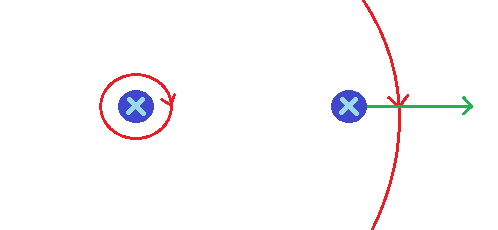
\includegraphics[scale=.50]{sameVortex.png}
\caption{The right hand rule tells us which direction the currents will swirl around a vortex pointing into the page. Then using Lorentz's law  at the second vortex, we can see that the second vortex will be pushed away. The same thing is happening from the current of the second vortex onto the first.}
\label{sameV}
\end{center}
\end{figure}

\begin{figure}[htbp]
\begin{center}
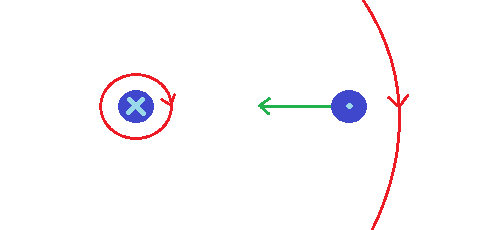
\includegraphics[scale=.50]{oppositeVortex.png}
\caption{The right hand rule tells us which direction the currents will swirl around a vortex pointing into the page. Then using Lorentz's law  at the second vortex, we can see that the second vortex will be pulled in this time. The same thing is happening from the current of the second vortex onto the first (although the second current flows in the opposite direction).}
\label{diffV}
\end{center}
\end{figure}

\subsection{Vortex-Defect Interactions}
The interaction between vortices and defects have been well-studied. Defects can be used to pin vortices and reduce dissipation. Defects can be impurities, vacancies, and inclusions. In one dimension they can be defects such as dislocations and irradiation tracks. Finally in three dimensions, they can be twin boundaries or stacking faults. The structure of atomic defects can have scattering properties which are either potential or magnetic type. Cooper pair-breaking caused by these defects has the effect of lowering the critical temperature. While studying these is important for pinning dynamics, it is the defecs which are on the order of several coherence lengths which are of interest to us. In three dimensions one can create columnar defects in the direction of the expected magnetic field. These have the strongest ability to hold on to vortices while causing the least amount of obstruction ~\cite{Kwok16}.

\subsection{Vortex-Wall Interactions}
The substrate is not always superconducting. It is also possible to embed non-superconducting components into the system. Since the super-current is suppressed in this system, There are many interesting effects to observe near these zones. First, a vortex near a magnetically neutral non-superconducting zone will be attracted to it. This can be seen as a type of "Venturi effect". Since the current flux must be conserved around a vortex, and there is not as much room for it to flow on the side closest to the wall, the current increases. A difference in current flux on opposing sides of the vortex then creates a force in the direction of the wall. The vortex is then pulled into the wall. The vortex will tend to remain there until pushed out by an external force. Two of the most common forces are external applied current and other vortices.

\begin{figure}[htbp]
\begin{center}
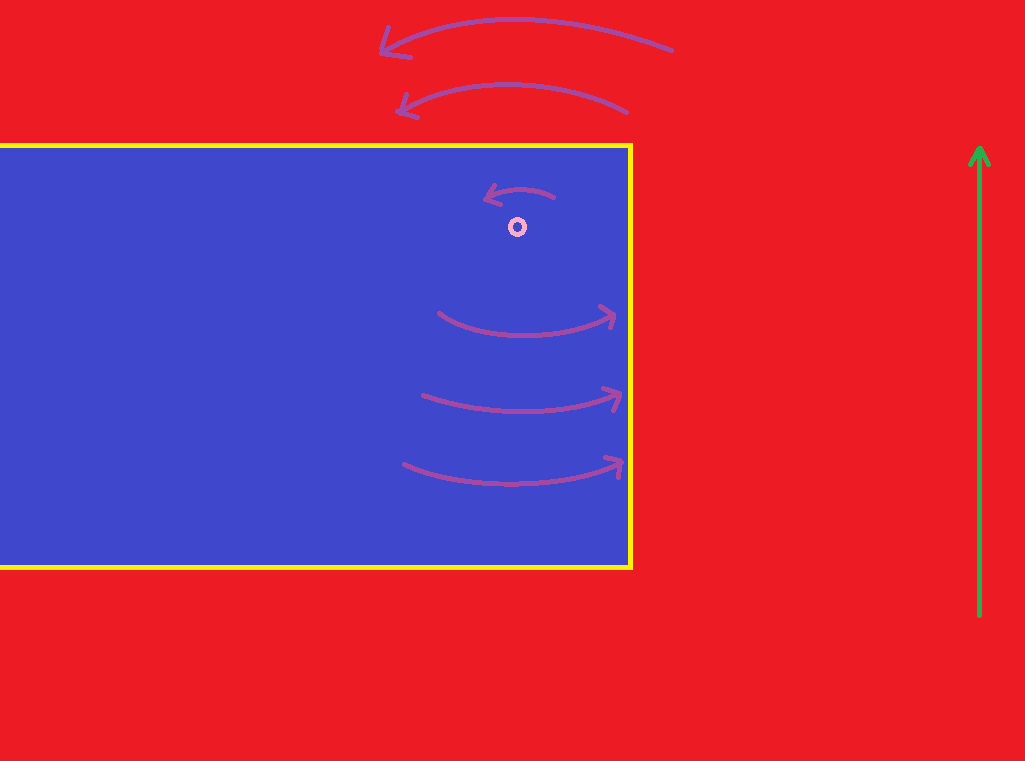
\includegraphics[scale=.50]{geometryInside.png}
\caption{Vortices (pink) will tend to get stuck inside inclusions (blue). That is because the supercurrent will travel faster outside of the inclusion, diminishing the amount of supercurrent inside. The vortex will therefore feel a force away from the boundary with the stronger superconductor.}
\label{geometryInside}
\end{center}
\end{figure}

\begin{figure}[htbp]
\begin{center}
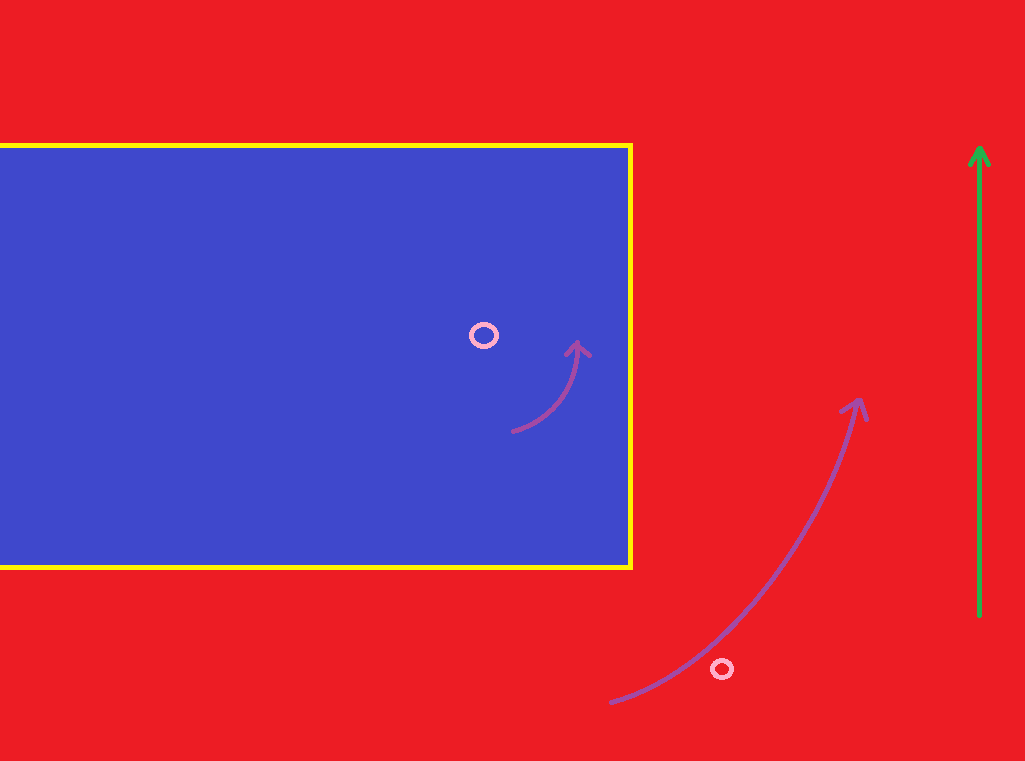
\includegraphics[scale=.50]{repulsion.png}
\caption{Once a vortex is stuck inside an inclusion, it will repel any other vortices which come near it.}
\label{repulsion}
\end{center}
\end{figure}

\section{Relevant Vortex studies}

Type 2 superconductors, while working at liquid nitrogen temperatures, have the problem of energy dissipation due to vortex dynamics. Therefore many geometric solutions are being worked on to try to slow down this energy loss. Here we focus on two of the most promising, vortex matching and funneling.

\section{Vortex Matching and $\delta T_c$ Pinning}
With improvements in nanotechnology, it has become easier to create grids of inclusions. These can be made by inserting nanorods of different critical superconducting temperature ($T_c$), pulsed laser deposition , by using ion beams to disrupt the superconducting lattice, or by using lithographic techniques.

Inserting nanorods of materials using bulk targets has is benefits and problems. These nanorods can be made to have different $T_c$ by controling the crystalinity or the amount of oxygen doping. \cite{Horii15} found a positive vortex-pinning effect due to the nanorods up to a magnetic field of 5 Tesla. They calculated the inter-vortex distance and designed a particular nanorod density. From there they were able to show that vortex-matching had a stronger pinning effect on the system. Varying the $T_c$ of the system is a powerful way to control the vortex dynamics.

Pulsed laser deposition of YBCO can extend the irreversibility of magnetic fields past the 10 Tesla marker. This was done by using BYTO additions to pin the fluxes. All of this is thanks to the increased availability of ordered nanosized oxide secondary phases in epitaxial thin films. This allows the tuning of material functionalities and has various applications including high temperature superconductors. They observed a large improvement to the critical current compared to untouched YBCO~\cite{Rizzo16}. Accurate placement of inclusions is important as inter-vortex forces are on the order of $1/r$.      

Ion beam etching can also be used to create the necessary inclusions. These antidot arrays can be made on thin films of Niobium Nitride using reactive dc sputtering. The antidot arrays are then created using a mask-aligner to do the ion-beam etching. They find experimental evidence for the observation that the maximum number of vortices which can be captured by an antidot of diameter d is
\begin{eqnarray}
n_s = \frac {d} {4 \xi(t)}, 
\label{}
\end{eqnarray}
where $\xi(t) = \xi_0 / \sqrt{1-t}$ and $t$ is a reduced temperature, typically in the range of $0.9 - 0.95$. They also found that vortices would become trapped in the antidots as well as in the interstices of the antidot lattice. This means that the critical current depends on the geometry of the lattice as well as the direction of current~\cite{Thakur09}. Multiple vortex antidots and inter-vortex trapping are important phenomenta when studying vortex matching. A theoretical basis for vortex matching has also been found. Berdiyorov et. al. ~\cite{Berdiyorov06} used the nonlinear Ginzburg-Landau theory to obtain all configurations for vortices in a grid of defects. They also find that vortices will pin in the inclusions and in between them. For small inclusions, they find only one vortex is trapped per hole. The hole radius and inter-hole distance determines the ability of multiple vortices to be forced into the holes. Like spheres in a box, The vortices prefer a triangular lattice as that affords the densest packing. If the pinning force of the holes becomes small enough, the lattices shift from the grid imposed quadratic lattice to a more natural triangular lattice. They find matching effects at whole and fractional magnatic field to hole ratios. Finally, they found their results to not agree with the Little-Parks theory of superconductors.

Lithographic (sputter etching) techniques were used to create arrays of submicrometere sized pinning arrays. These were compared to simulated $J_c$ curves using the time dependent Ginzburg Landau model. They found that the critical current exibited maxima at the expected matching fields at 2.3 degrees Kelvin. The critical current was considerably larger than systems without antidot arrays~\cite{Sabatino10}.
It is important to have a physical temperature at which these phenomena occur as most Ginzburg-Landau simulations only describe temperature in relation to $T_c$.

\section{Vortex Jamming and Geometric Pinning}
Another way to increase the depinning current of a system is to get the vortices to pin each other. This jamming effect can be accomplished by manipulating the geometry of the system they must past through. Different geometric strategies have been tried including simple funnels, diamonds, and conformal maps. Vortex ratchets and fluxon pumps are also of great interest in the superconducting world. These use diode-like geometries to keep vortices going in one direction. These effects can be seen even with a symmetric force such as an alternating current.  

Computer simulations have been popular in demonstrating the usefulness of vortex ratchets. Within these ratchets, vortices will go through certain phases depending on the strength of the magnetic field. These phases are known as triangular, smectic, disordered, and square~\cite{Lu06}. They showed that sawtooth ridges which modulate the z-component of a superconductor can have a similar effect as triangular modulations in the x and y-components. They used a Langevin model to simulate the vortices, which starts to become unphysical as the vortex density increases.  

The optimal size of the funnel tip is such that only one vortex can pass at a time due to vortex-vortex repulsion forces. Reichhardt et. al.~\cite{Reichhardt10} , through the help of simulations, observed that the sum of the vortex velocities remains constant with increasing magnetic field. They highlight the similarities to a granular hopper, decreasing the width of the hopper aperture decreases the flow of grains. They found that as the number of vortices increases, the pinned vortex structure becomes larger and harder to deform. This then keeps individuals from passing through the bottleneck.

Fluxon pumps can be used to extract useful work from a fluctuating environment. The vortex ratchet can be used as a fluxon rectifier. These could be used as fluxon lenses to concentrate or disperse magnetic fields. These would have various uses including dispersing trapped flux in SQUID magnetometers. But to get the desired effects, the frequency must hit the appropriate resonance region~\cite{Wambaugh99}. This means not only the right frequency for the geometry, but also the correct temperature (i.e. random motion). Thermal noise had to be kept low in the pinning systems. Like sand in an hourglass, minor turbulence has a large effect on the ability of vortices to stick. They again back up the idea that the more fluxons one has, the more their motion will be restricted.

Vortices travelling through constricting lattices can also be used to study the dynamics of interacting particles travelling through confining potentials. Yu et. al. found that with the correct geometry, vortices would begin moving as the external magnetic field varied~\cite{Yu10}. They found strong matching effects between the vortex distribution and the constriction lattice. By tailoring their diamond shaped channel, they could pick their confining potential. The angle of the wall has a strong effect on the ability of the system to be immobilized.

We built upon previous GLGPU research in geometric pinning. In order to simulate geometrical constraints and voids of various shapes we impose appropriate internal boundary conditions or use unstructured grid discretizations~\cite{Kwok16}. The boundary conditions are imposed via picking no current (open) boundaries which simulate insulating inclusions~\cite{Sadovskyy14}. Multiple types of tesselations are also possible, including checkerboard, or less standard Voronoi tesselations. These are useful for polycrystalline thin superconducting films with variations of $T_c$.

\section{GLGPU overview}
GLGPU is a GPU-based Jacobi solver for the time-dependent GL equations. It was designed to solve mesoscale problems which arised in superconductor design. Instead of treating the vortices as elastic strings in a viscous medium, it focuses on the underlying order parameter. This allows for correct interactions between pairs of vortices, vortices and inclusions, and allows the vortices to split up and rejoin. To model the system accurately, we need to take into account the Ginzburg Landau function at a microscopic resolution as a complex valued scalar field. The amplitude of this field is related to the supercondonductivity density, while the phase is related to the current of the system (after a gauge transformation). Through careful optimization, the system size can be made large enough to encompass many vortex interactions and complicated non-superconducting architectures. Physical pinning defects are simulated as modulations of the superconductor's critical temperature. The simulation works by first integrating the GL equations forward in time, then solving the Poisson equiation to find the electric and magnetic fields. There are also noise correlation terms to simulate thermal effects~\cite{Sadovskyy14}.

\subsection{stable GLGPU system}
The particular Ginzburg Landau equations which were used are designed to be particularly stable. In appendix 1, we explore the limits of this system and find it works for all relevant currents. These current equations were :
\begin{eqnarray}
J_N = -\sigma [(1/c) \partial_t A + \nabla \mu ]
\label{currentEq1}
\end{eqnarray}
and
\begin{eqnarray}
J_S = -\frac{e}{2m} [\psi*(i\hbar \nabla + \frac{2e}{c} A) \psi + c.c.],
\label{currentEq2}
\end{eqnarray}
where $\nabla A = 0$, $\sigma$ is the conductivity, $\mu$ is the scalar potential, $A$ is the vector potential, $e$ is electron charge, $c$ is the speed of light, and $m$ is electron mass. To help with stability, the Crank-Nicolson integration scheme and the linearization of the $|\psi|^2\psi$ term were done. An explicit integration would be subject to numerical instabilities.

\subsection{Boundary conditions}

There are two types of boundary conditions relevant to this system. They are quasi-periodic and open. On a quasi-periodic boundary, cells are treated the same as they would be in the middle of the system. The only thing that one needs to keep track of is the phase jump at the boundary. In other words, only the amplitude of the order parameter is really periodic. The open boundary refers to the Neumann boundary conditions. These mean that there is no current perpendicular to the boundary. Specifically;
\begin{eqnarray}
\overrightarrow n (\nabla - i \overrightarrow A)\psi = 0 ,
\lable{}
\end{eqnarray}
where $\overrightarrow n$ is the unit normal vector. For our studies, we stuck with quasi-periodic boundary conditions in the direction of current.



\section{Results}
Being such a general code, there were many possible areas of study regarding this code. We found promissing results in two general areas, grids of inclusions and super conducting-conducting funnels with higher $T_c$. We characterize these situations by looking at their responses to changes in voltage, magnetic field, and geometry. There is an important choice that we made when determining the critical current as there is a inherent hysteresis in the system. We had two options when ramping the current. It could either have been ramped up, Starting with no movement and pushing the current until the vortices became dislodged. The second option was to ramp the current down. That is start with moving vortices and slowly decrease the current until the vortices become lodged. In the end we went for the second option due to the dynamics of the system. Vortices tend to start out placed not according to the lowest energy state, but instead randomly according to whatever starting seed was selected. By forcing the vortices to move around first, we get a more natural state before the depinning current is found. In figure ~\ref{hysteresis} we quantitatively demonstrate the difference.

\begin{figure}[htbp]
\begin{center}
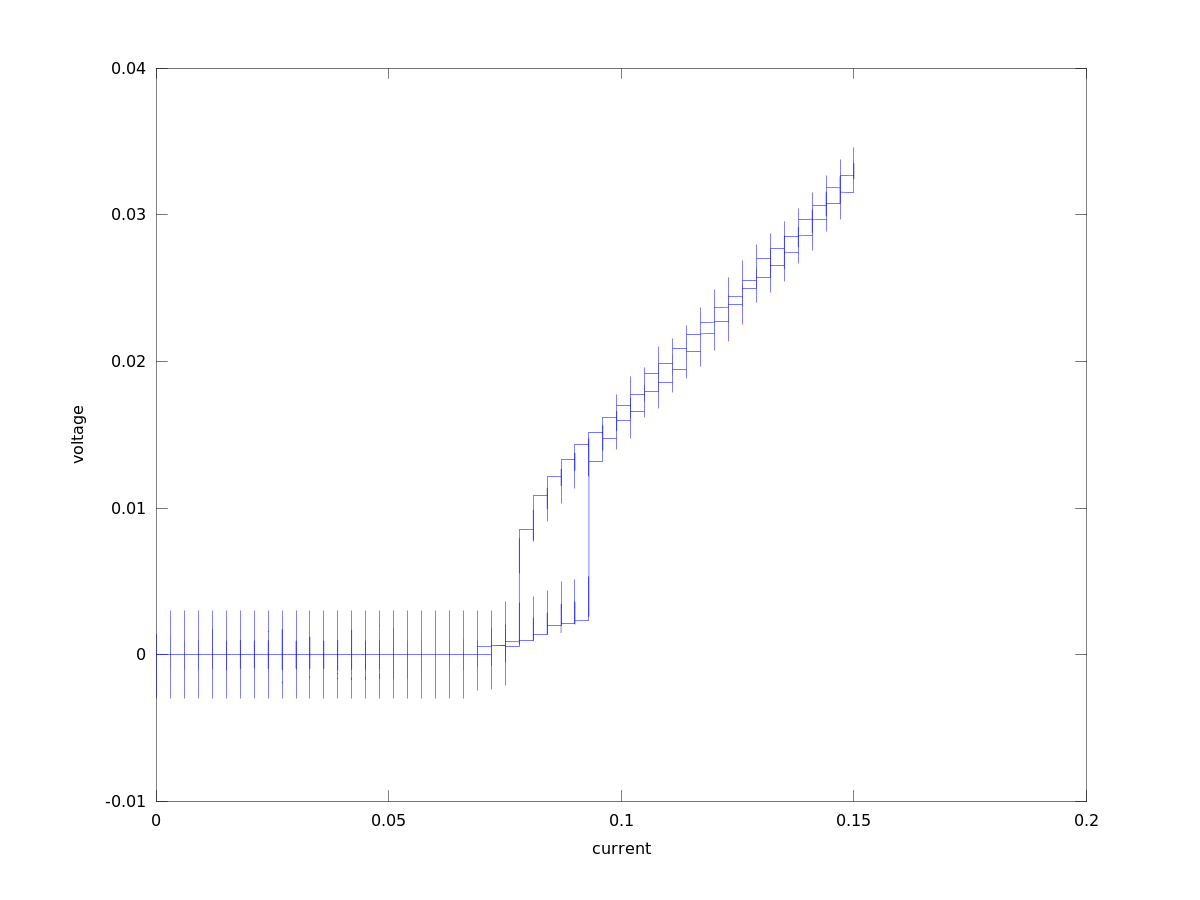
\includegraphics[scale=.50]{JvV.png}
\caption{ Overlapped are the current vs voltage for two systems, one with the current ramped up and one with the current ramped down. Upper one is the current being ramped down, while the lower one is the current ramped up.}
\label{hysteresis}
\end{center}
\end{figure}


\subsection{Grids}
Inclusions in the superconductive substrate can be used to contain vortices (up to a certain current). If these vortices do not move, then they are not draining energy from the system. The first thing we needed to show was that vortices preferred to be trapped in inclusions which were around the same size as they were. If the inclusion size is increased, we see that at some point we start to trap 2 vortices per inclusion. Trapping a vortex requires that the force due to external current and other vortices be less than the superconducting destruction force. The superconducting destruction force is due to the energy of a superconducting system below Tc Being lower than a non-superconducting system below Tc. The second effect we were looking for was vortex matching resistance. Vortices have quantized magnetic flux. This means that for a certain applied field, we can predict the number of vortices. If some vortices are moving and some are pinned, the moving ones will push on the pinned ones as they pass by. If instead we have as many vortices as we have inclusions, after a certain relaxation period, vortices will all be pinned and the system will be more stable. As shown in Fig.~\ref{HDF} we were able to show both of these effects. In the X direction, we see that the optimal radius for an inclusion is 2. In the Y direction, we see a sharp drop in critical current at m=1. This is because as soon as we are above the 1-to-1 ratio, we start to have rogue vortices which will move. As the magnetic field is increased, we start to see that there islands of stability where multiple vortices can fit on the same inclusion. There is also a quadratic relation between the magnetic ratio and the size of the vortices in terms of optimal conditions.

\begin{figure}[htbp]
\begin{center}
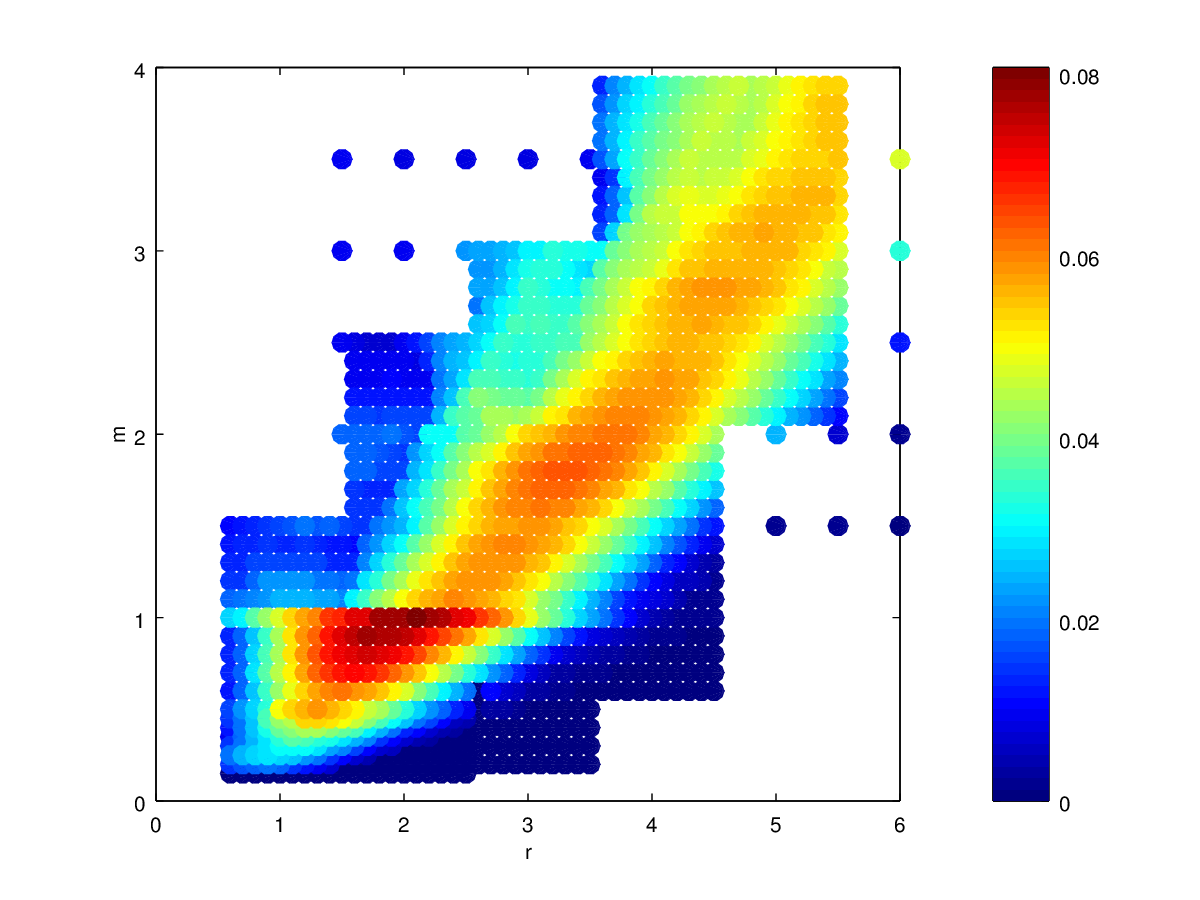
\includegraphics[scale=.50]{HDFinal.png}
\caption{ This is a superposition of 100+ simulations with different parameters. The critical current of each simulation was shown using color. On the X-axis is the radius of each inclusion in the system. On the Y axis m is the ratio of number of vortices per inclusion. The colorbar stands for critical current. In other words, the redder a zone is, the better it holds on to vortices, the higher the current can be before the vortices begin to slip.}
\label{HDF}
\end{center}
\end{figure}

\section{Funnels}
The same way that energy is gained when a vortex goes into a lower superconducting state, energy is lost if it tries to go into a higher superconducting state. Also, since more current can travel through the superconducting system, we get the opposite of the venturi effect. This also helps to keep vortices out. Using this logic, we created superconducting zones with higher $T_c$ that can be used to guide vortices. Indeed, increasing the aperture size increases the ease of which the vortices can travel ~\ref{AvR}.

\subsection{Description}
The magnetic field was kept such that the number of vortices filled 50\% to 80\% of the substrate. It was pointed into the board such that the current pushed the vortices into the funnel. The current was started at an amount large enough to guarantee vortex movement, even if it also meant that vortices went through the walls at first. The current was then slowly relaxed in enough timesteps to make sure that each configuration had enough time to stabilize. The number of current configurations had to balanced against practicallity. Ideally, we would use an infinite number of current configurations, but that would take an infinite ammount of time to simulate. Instead we tried to keep the simulation times at less than 24 hours.

\subsection{Analysis}
In general, the simulations performed as expected. The smaller the aperture, the better a system can hold on to vortices. This is up to a point which where even 1 vortex can no longer slip through. Steeper angles also improved the jamming performance of each system. The dependence did not seem to be linear in y-position of the funnel, or in angle. When looking at the magnetic dependence of the critical current, it is clear that more vortices increase the critical current of the system.
\begin{figure}[htbp]
\begin{center}
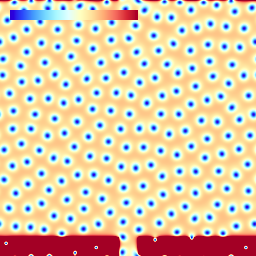
\includegraphics[scale=.50]{ratchetNoAngle.png}
\caption{ The amplitude of the complex order parameter. in yellow is the background superconductor, In red is the superconductor wall, and the blue dots are the vortices. In green is the parameter of interest. In this case, we have a flat obstruction which forces vortices through a narrow gap.}
\label{noAngle}
\end{center}
\end{figure}

\begin{figure}[htbp]
\begin{center}
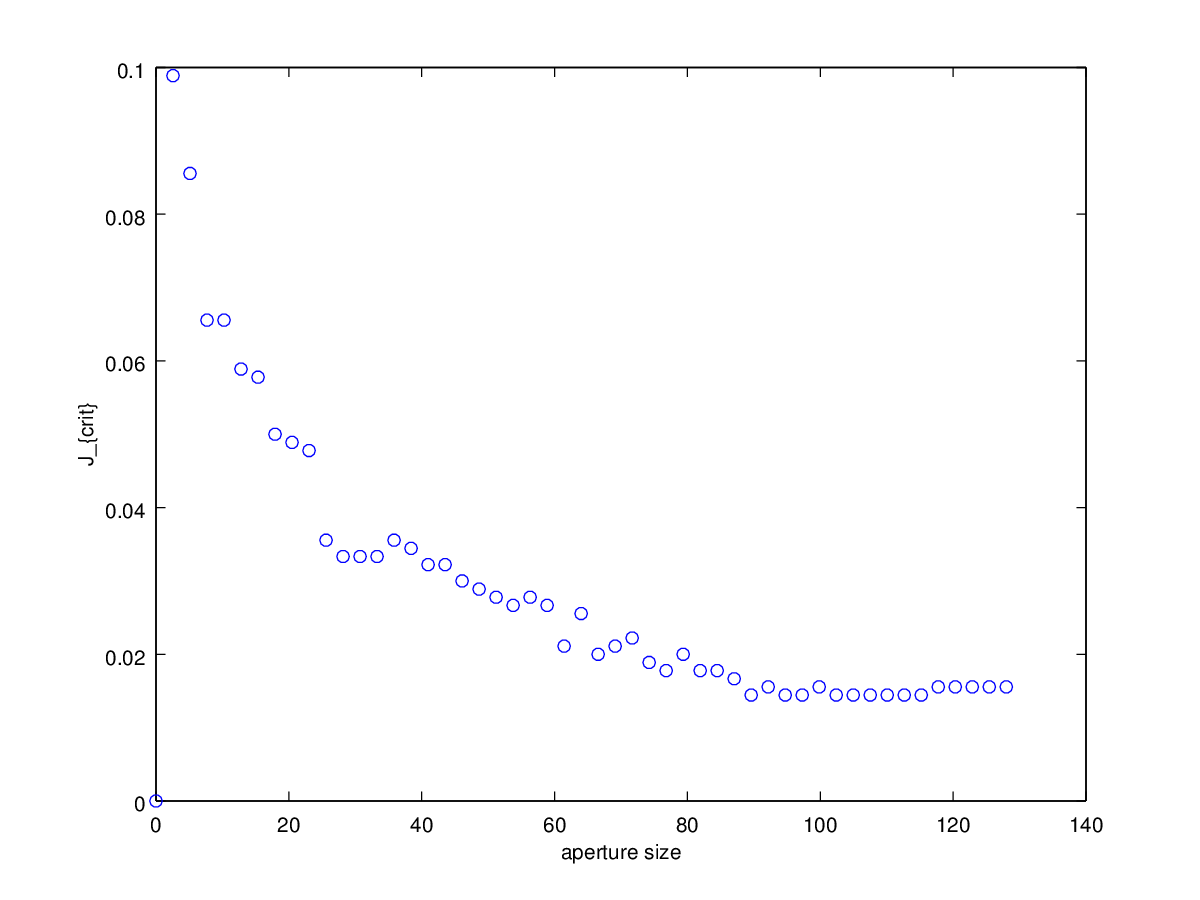
\includegraphics[scale=.50]{flatScan.png}
\caption{ 50 values of aperture were run in this simulation. The resulting current was analyzed to find the critical current . As the aperture is increased, the ability to hold the vortices still is diminished. }
\label{flatScan}
\end{center}
\end{figure}


\begin{figure}[htbp]
\begin{center}
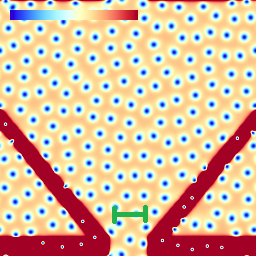
\includegraphics[scale=.50]{normalX.png}
\caption{ The amplitude of the complex order parameter. in yellow is the background superconductor, In red is the superconductor wall, and the blue dots are the vortices. In green is the parameter of interest. In this case it is the size of the aperture which was varied. }
\label{normalX}
\end{center}
\end{figure}

\begin{figure}[htbp]
\begin{center}
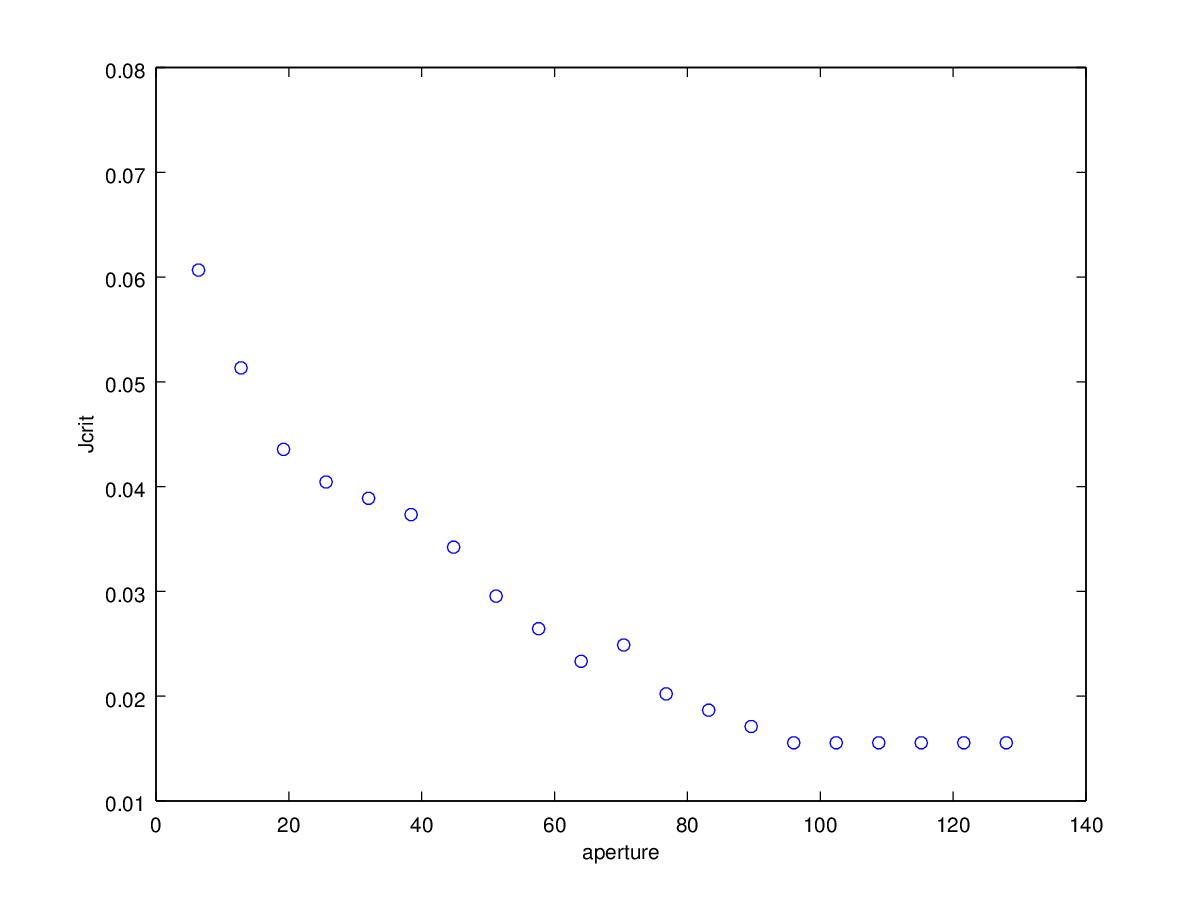
\includegraphics[scale=.50]{normalXscan.png}
\caption{ 50 values of aperture were run in this simulation. The resulting current was analyzed to find the critical current . As the aperture is increased, the ability to hold the vortices still is diminished. }
\label{normalXscan}
\end{center}
\end{figure}

\begin{figure}[htbp]
\begin{center}
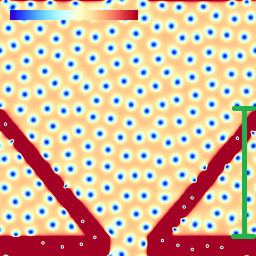
\includegraphics[scale=.50]{normalY.png}
\caption{ The amplitude of the complex order parameter. in yellow is the background superconductor, In red is the superconductor wall, and the blue dots are the vortices. In green is the parameter of interest. In this case it is the point on the Y-axis at which the funnel attaches and therefore the angle which varies. }
\label{normalY}
\end{center}
\end{figure}

\begin{figure}[htbp]
\begin{center}
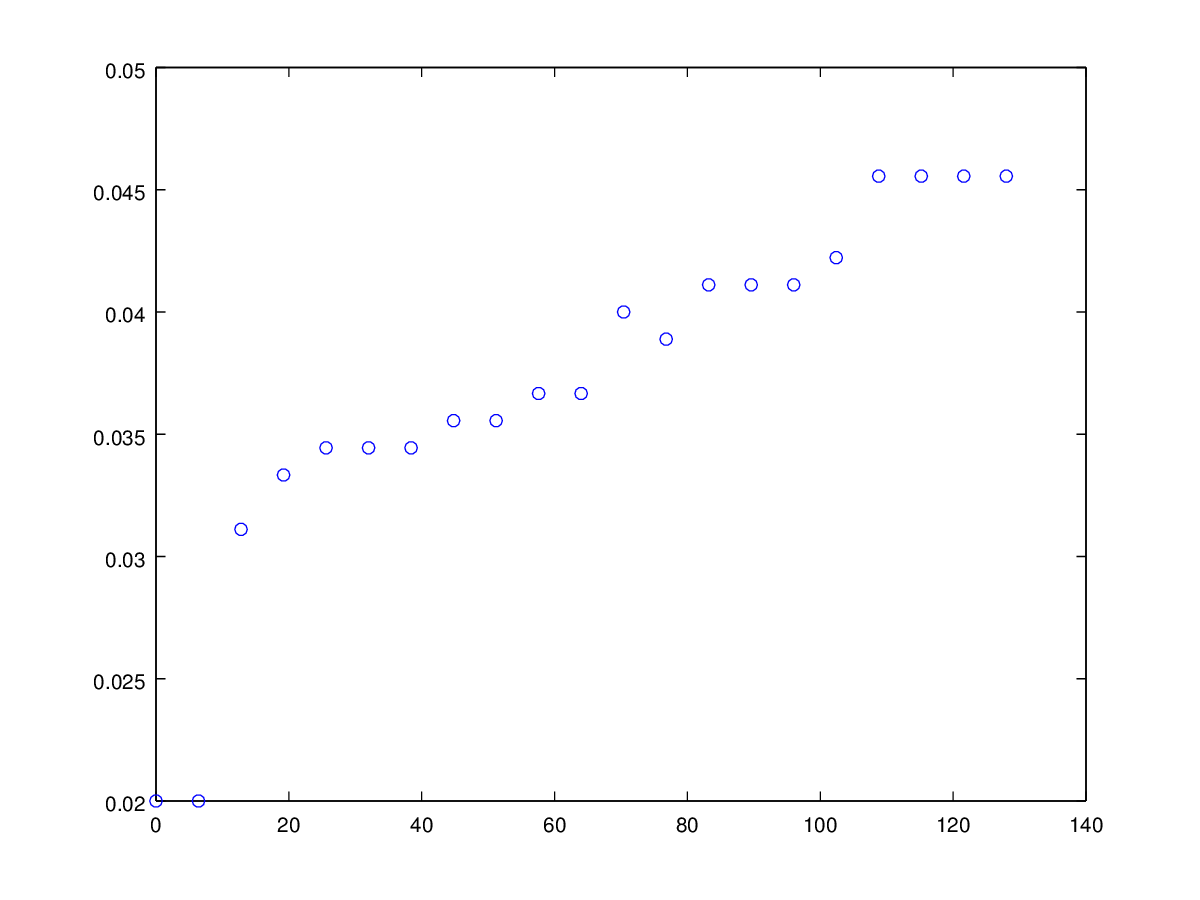
\includegraphics[scale=.50]{normalYscan.png}
\caption{ 50 values of aperture were run in this simulation. The resulting current versus voltage information was analyzed to find the critical current . As the angle of the slope is increased, the vortices were more easily jammed. }
\label{normalYscan}
\end{center}
\end{figure}


\begin{figure}[htbp]
\begin{center}
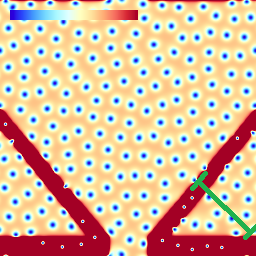
\includegraphics[scale=.50]{normalAngle.png}
\caption{ The amplitude of the complex order parameter. in yellow is the background superconductor, In red is the superconductor wall, and the blue dots are the vortices. In green is the parameter of interest. In this case the angle is held constant while the x and y attachments are varied. }
\label{normalAngle}
\end{center}
\end{figure}

\begin{figure}[htbp]
\begin{center}
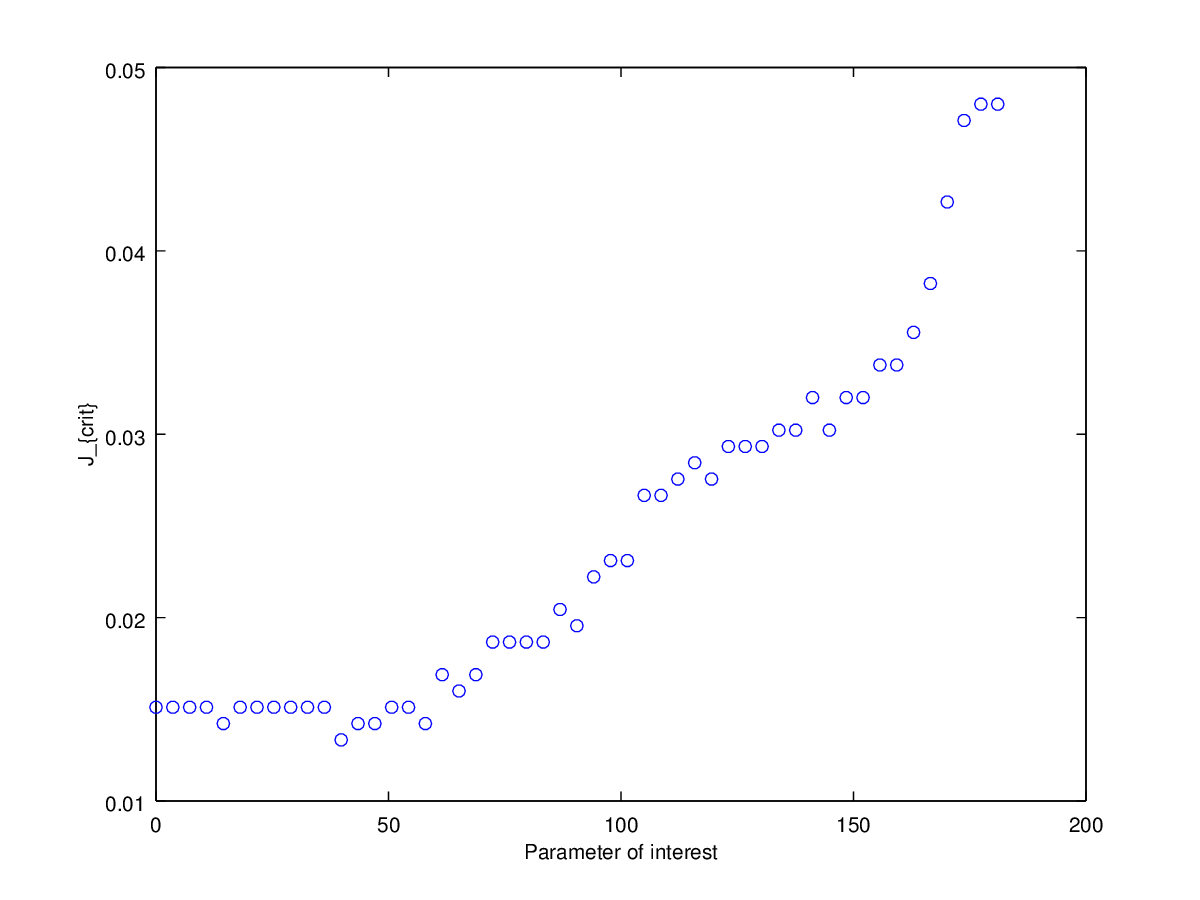
\includegraphics[scale=.50]{constantAngle.png}
\caption{ This is a scan of the parameter of interest versus the critical current. The x-postition and y-position of the funnel were moved uniformly as to keep the angle constant. }
\label{constantAngle}
\end{center}
\end{figure}


\begin{figure}[htbp]
\begin{center}
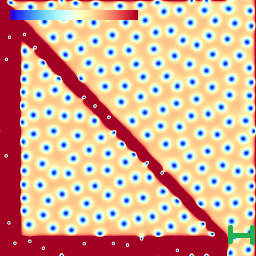
\includegraphics[scale=.50]{oneSidedDone.png}
\caption{ The amplitude of the complex order parameter. in yellow is the background superconductor, In red is the superconductor wall, and the blue dots are the vortices. In green is the parameter of interest. In this case it is the size of the aperture which was varied. }
\label{oneSidedX}
\end{center}
\end{figure}


\begin{figure}[htbp]
\begin{center}
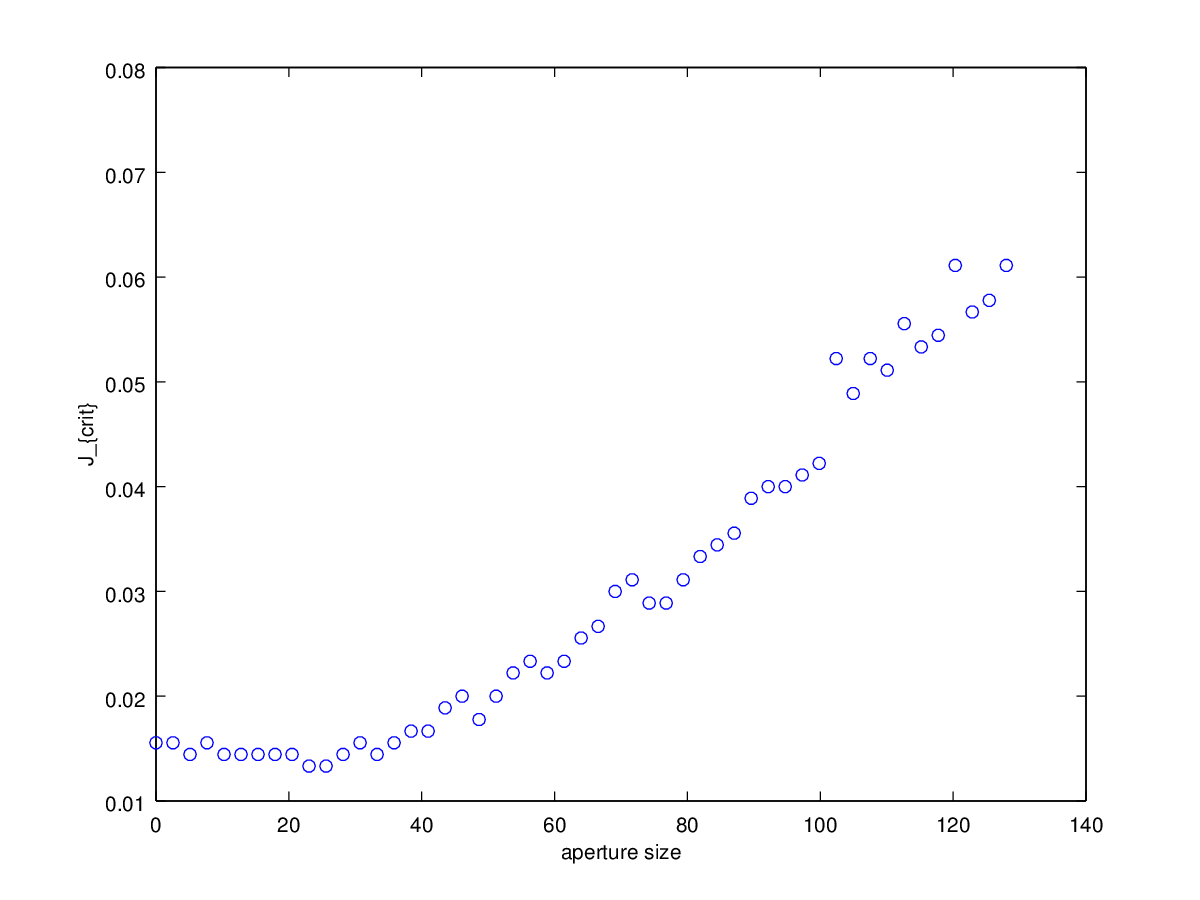
\includegraphics[scale=.50]{oneSidedAperture.png}
\caption{ 50 values of aperture were run in this simulation. The resulting current versus voltage information was analyzed to find the critical current . As the aperture size is increased, the vortices are less restrained. }
\label{normalYscan}
\end{center}
\end{figure}

\begin{figure}[htbp]
\begin{center}
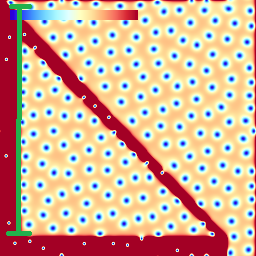
\includegraphics[scale=.50]{oneSidedY.png}
\caption{ The amplitude of the complex order parameter. in yellow is the background superconductor, In red is the superconductor wall, and the blue dots are the vortices. In green is the parameter of interest. In this case it is the point on the Y-axis at which the funnel attaches and therefore the angle which varies.}
\label{oneSidedY}
\end{center}
\end{figure}

\begin{figure}[htbp]
\begin{center}
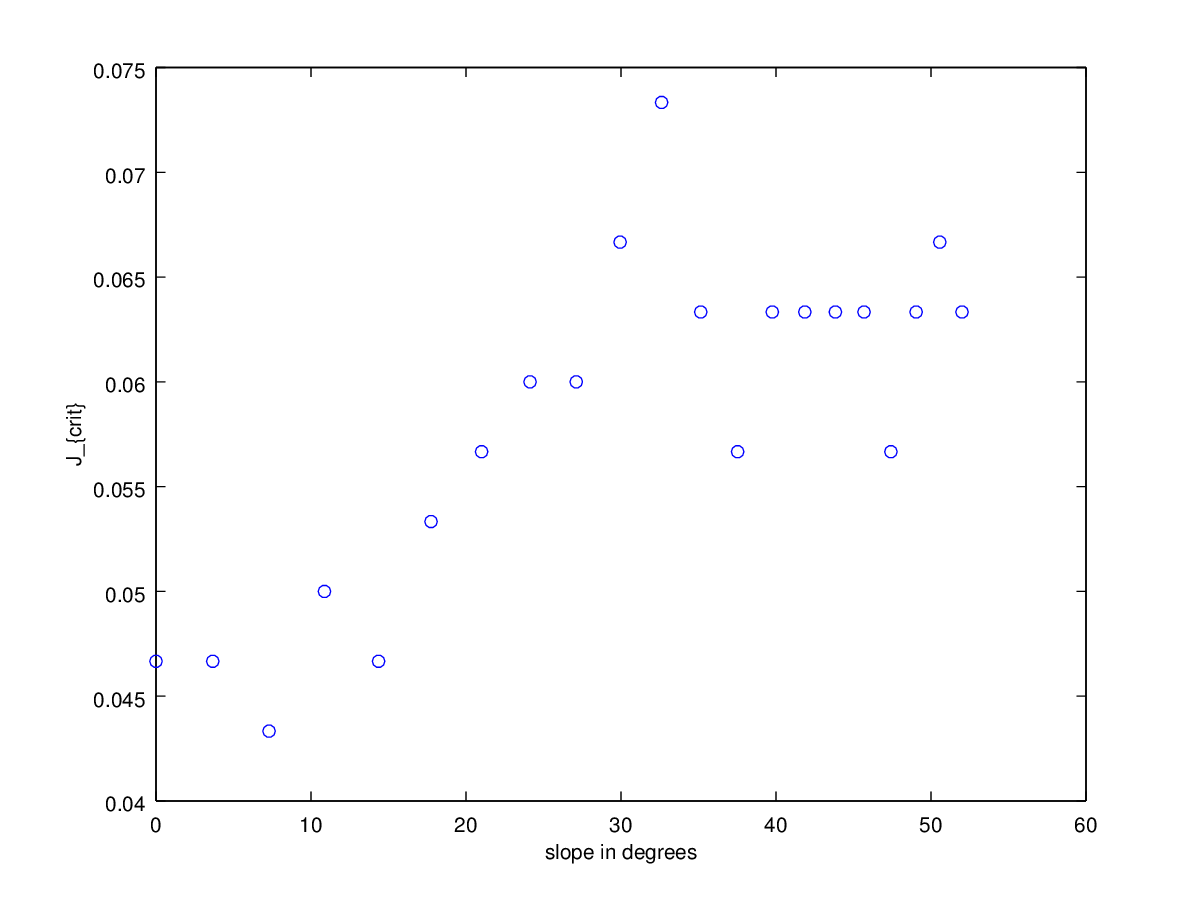
\includegraphics[scale=.50]{oneside-angle-Scan.png}
\caption{ 50 values of aperture were run in this simulation. The resulting current versus voltage information was analyzed to find the critical current . As the one slope is increased, the jamming effect becomes more pronounced. }
\label{normalYscan}
\end{center}
\end{figure}

\begin{figure}[htbp]
\begin{center}
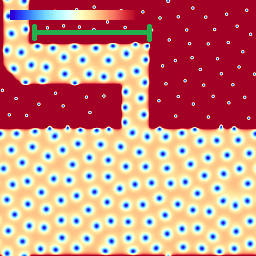
\includegraphics[scale=.50]{oneKinkDone.png}
\caption{ The amplitude of the complex order parameter. in yellow is the background superconductor, In red is the superconductor wall, and the blue dots are the vortices. In green is the parameter of interest. In this case it is the length of the "turn" which is being varied.}
\label{oneSidedY}
\end{center}
\end{figure}

\begin{figure}[htbp]
\begin{center}
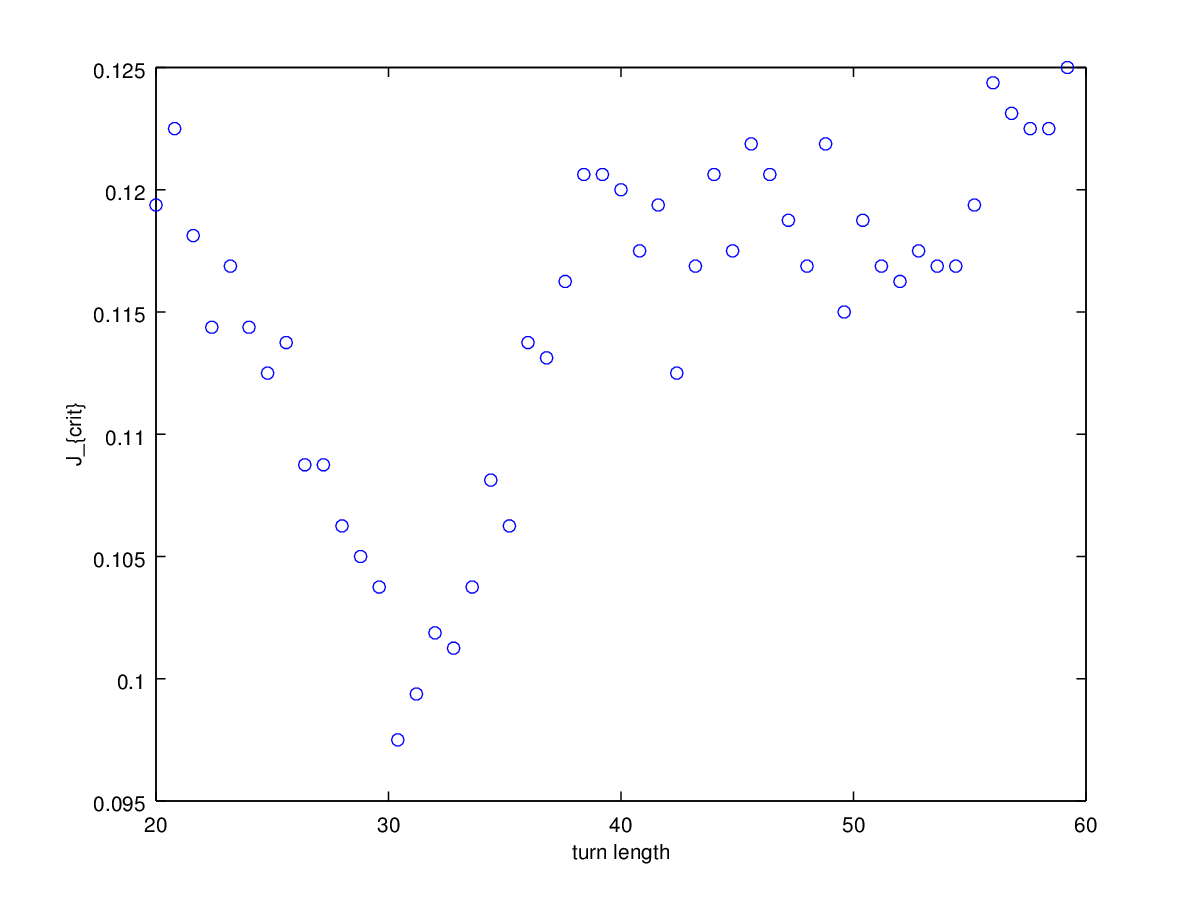
\includegraphics[scale=.50]{kinkScan.png}
\caption{ 50 values of the turn length were run in this simulation. The resulting current versus voltage information was analyzed to find the critical current .  }
\label{normalYscan}
\end{center}
\end{figure}



\begin{figure}[htbp]
\begin{center}
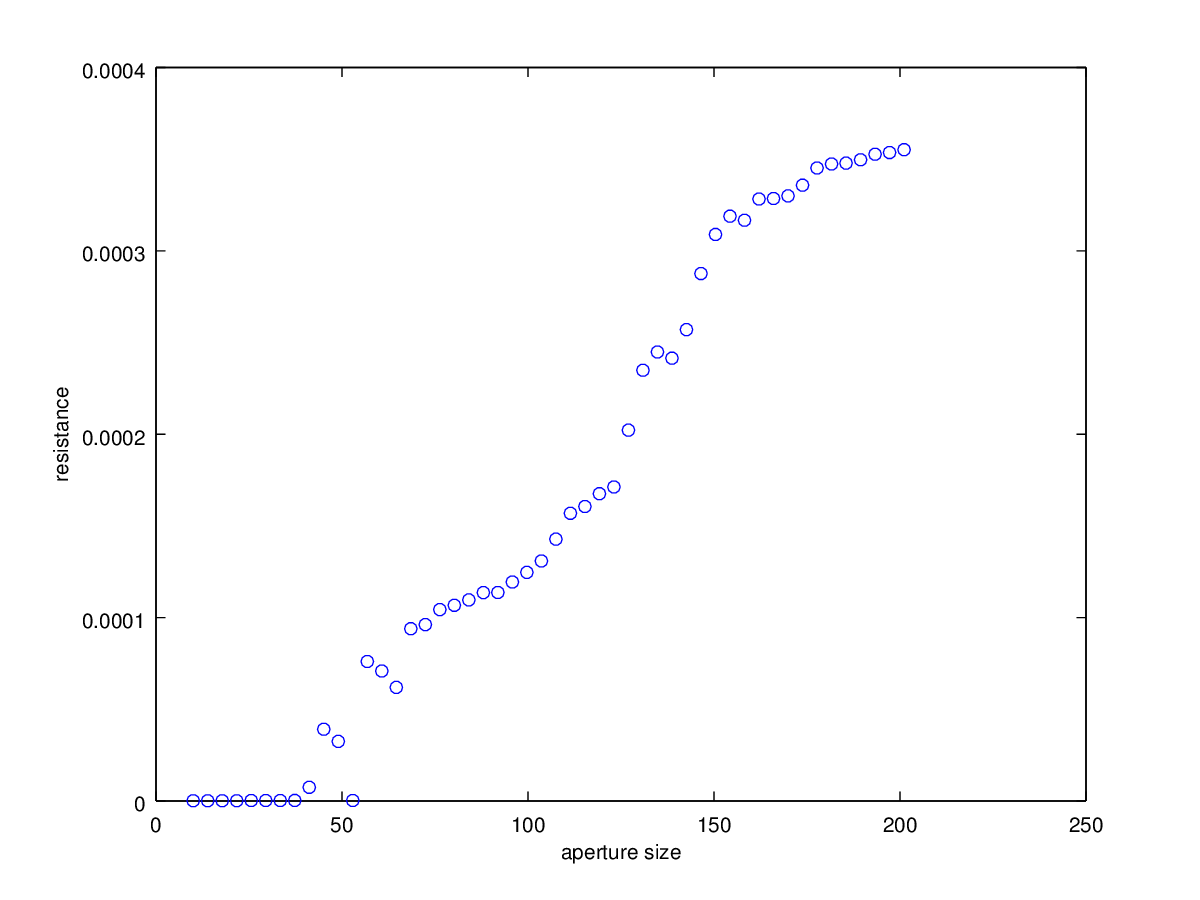
\includegraphics[scale=.50]{AvR.png}
\caption{ We can also study how the aperture size hampers vortex movement once they have already been depinned. This is a resistance plot of the constant y-position funnel. On the X axis is the size of the aperture, Y axis is the superconductive resistance. }
\label{AvR}
\end{center}
\end{figure}

\begin{figure}[htbp]
\begin{center}
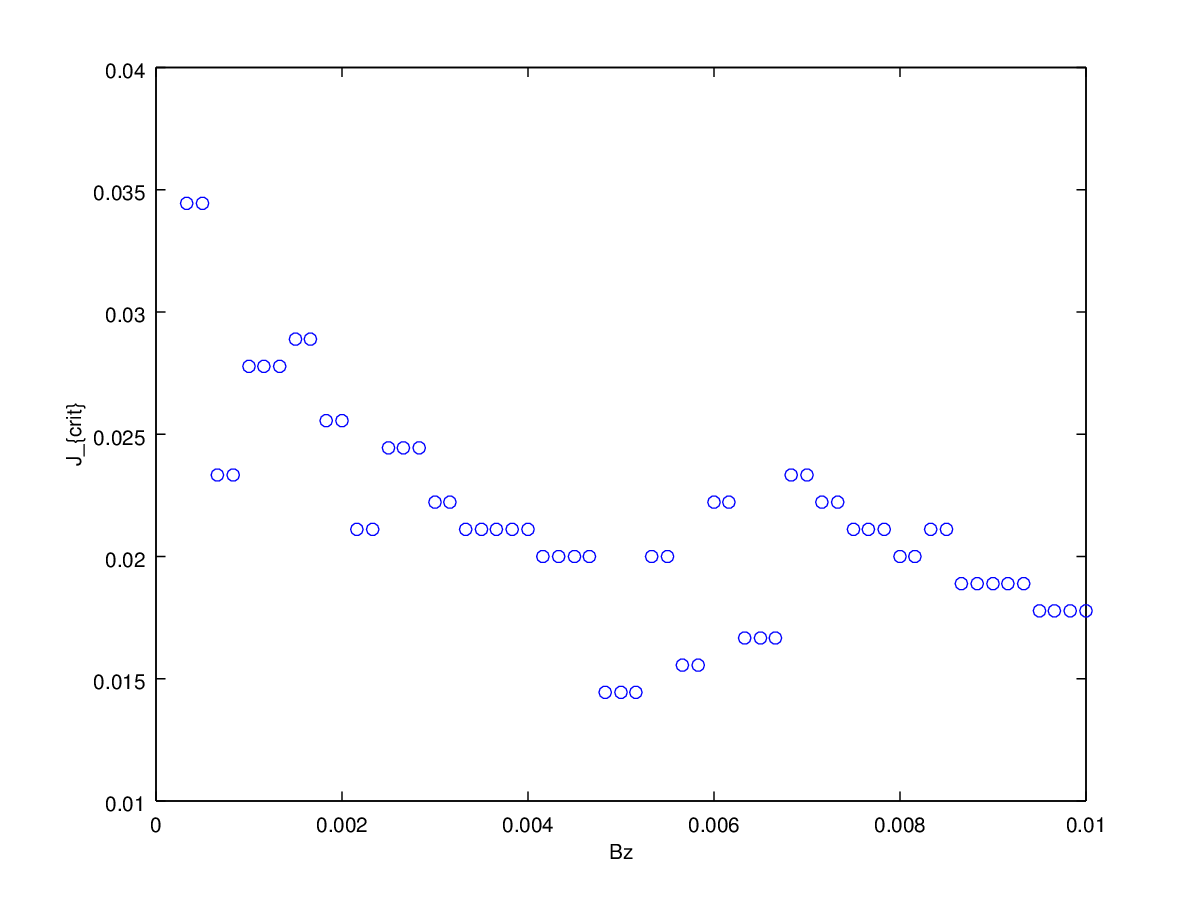
\includegraphics[scale=.50]{angleBz.png}
\caption{ 50 values of the magnetic field angled system. The resulting current versus voltage information was analyzed to find the critical current .  }
\label{angleBz}
\end{center}
\end{figure}


\begin{figure}[htbp]
\begin{center}
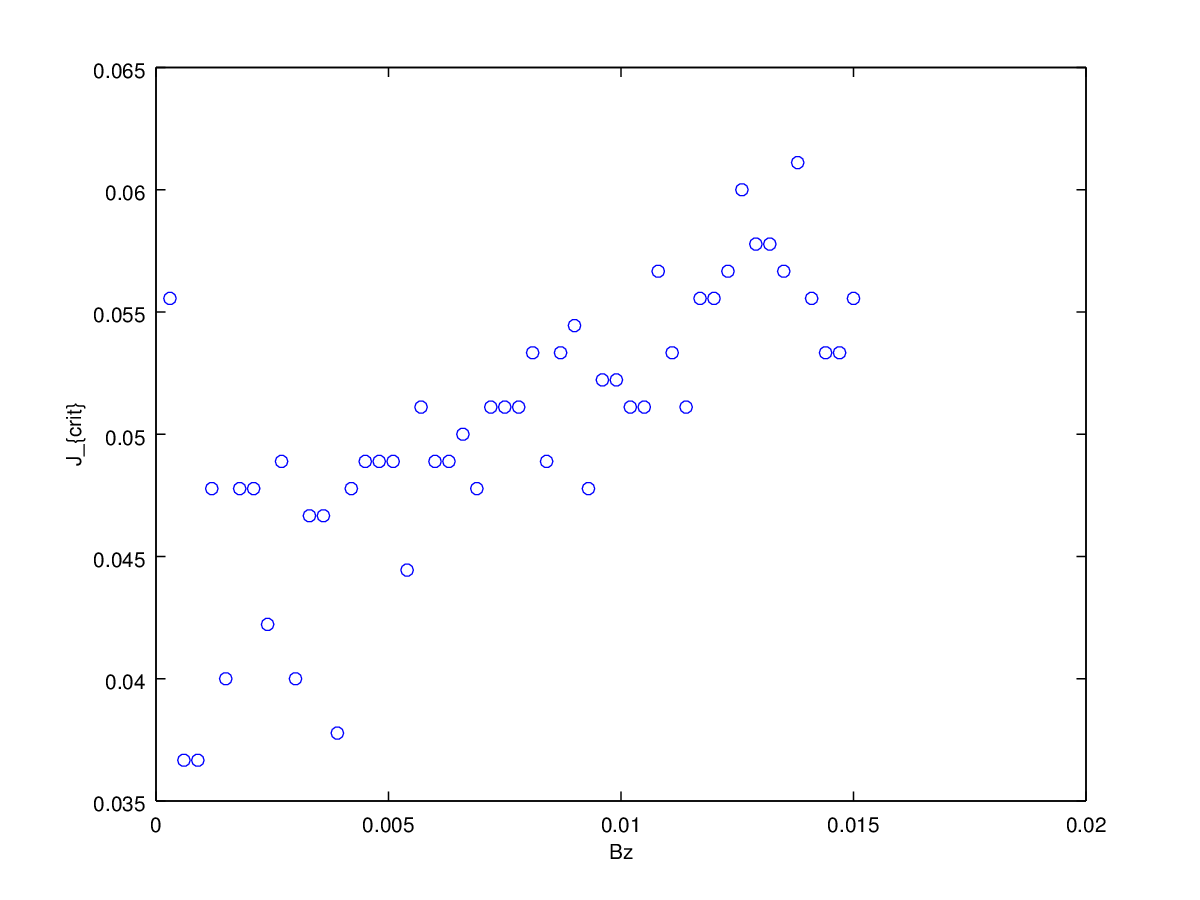
\includegraphics[scale=.50]{emptyBz.png}
\caption{ 50 values of the magnetic field were studied for the empty diamond system. The resulting current versus voltage information was analyzed to find the critical current .  }
\label{emptyBz}
\end{center}
\end{figure}

\begin{figure}[htbp]
\begin{center}
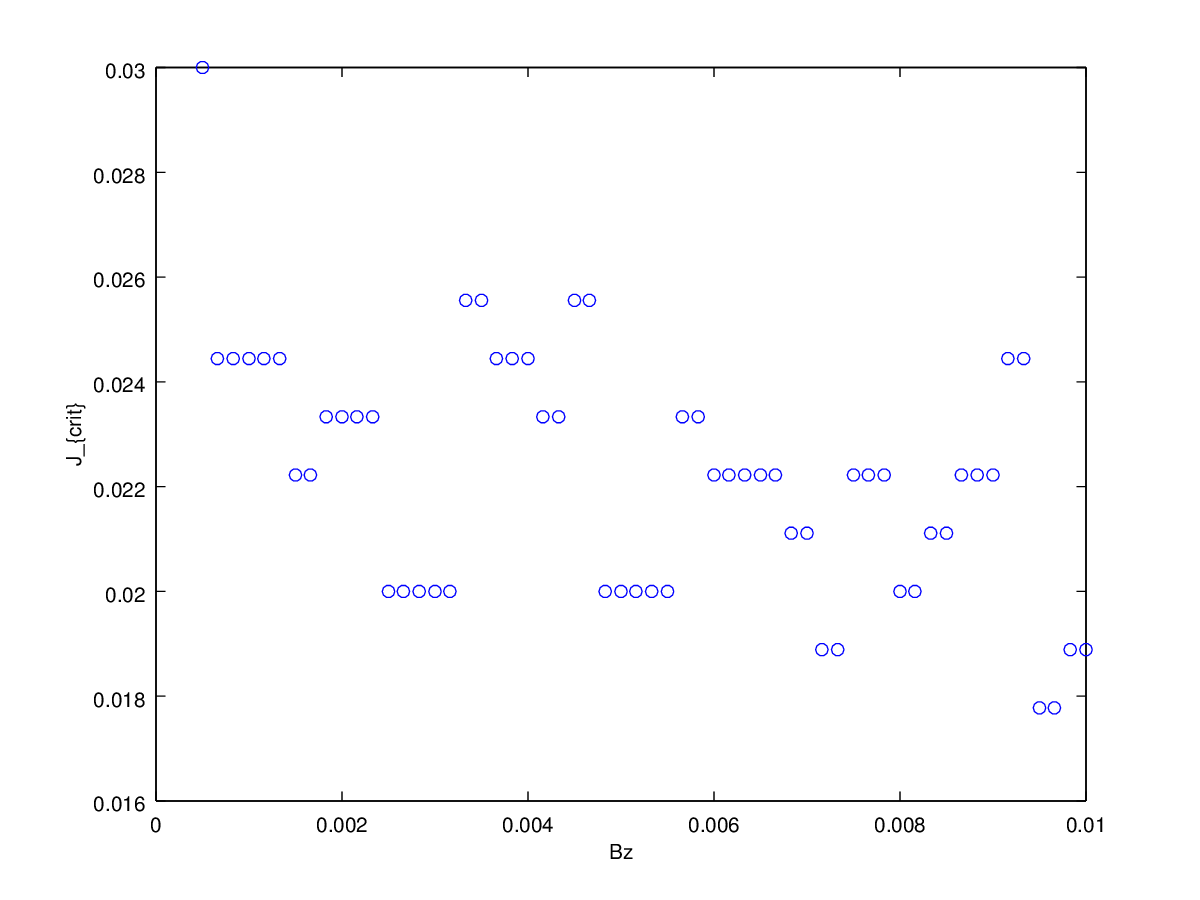
\includegraphics[scale=.50]{flatBz.png}
\caption{ 50 values of the magnetic field were studied for the flat system. The resulting current versus voltage information was analyzed to find the critical current .  }
\label{flatBz}
\end{center}
\end{figure}

\begin{figure}[htbp]
\begin{center}
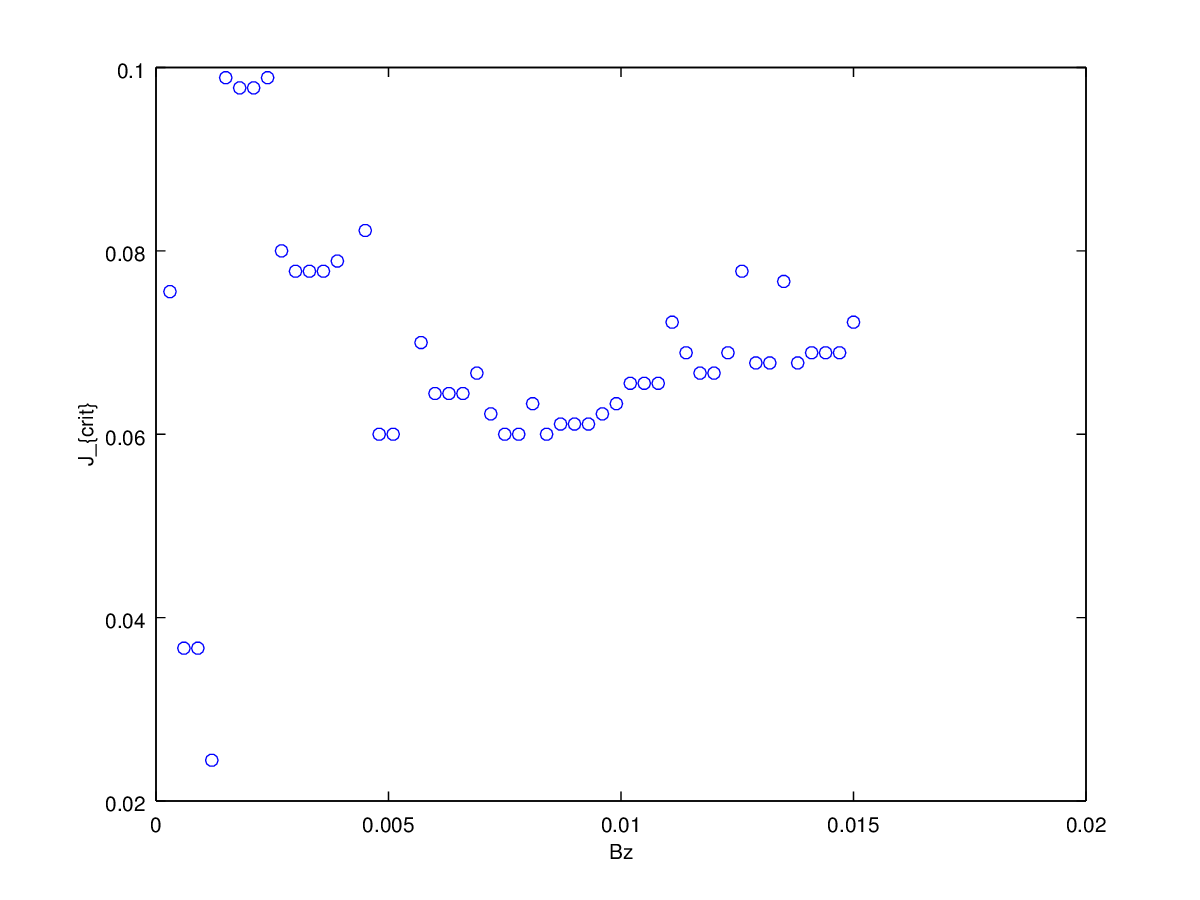
\includegraphics[scale=.50]{oneSideBz.png}
\caption{ 50 values of the magnetic field for the one sided system. The resulting current versus voltage information was analyzed to find the critical current .  }
\label{oneBz}
\end{center}
\end{figure}

To conclude, we have explored multiple systems with the use of the GL program. We showed that if the number of inclusions matches the number of vortices, the system jams and we have much lower resistance due to vortex motion. We have also explored many funnel systems which are currently being tried out experimentally throughout the superconduction community. We showed that vortex jamming is a function of the angle of the funn
el, the size of the aperture, and the amount of vortices.

 
		% file with references
\chapter{Variable Range Hopping}		% chapter 1
\label{theorychap}

\section{History}
In 1937, Nevill Mott and Rudolf Peierls explained why some materials which should have been conductors, acted as insulators. This was due to electron-electron interactions, which is not taken into account in band theory ~\cite{mott72}. From there, Miller and Abrahams proposed a network resistor model which Efros and Schklovskii built on ~\cite{efros75}. Because of the dynamic complexity of even a small system (a 10 by 10 system can have $2^{100}$ configurations) simulations are a large part of modern electron hopping studies ~\cite{kirkengen09}. The theory has gotten more consise over time. For the sake of simulation, much of it can be compressed into equation~\ref{probability}.

Transport through a quantum dot which is weakly coupled to two conducting leads is dominated by the electron-electron interaction ~\cite{Glazman05}. When the thermal energy is not enough to overcome the charging energy of the dot, coulomb blockade takes over and resistance is increased. At low enough temperatures, the Kondo effect takes over. That is when the magnetic field of the electrons starts to matter energy-wise. At that point, electrons start to prefer states where they are anti-parallel.

Kinetic monte carlo methods are useful when simulating condensed matter systems which include time evolution. There are two types, rejection and rejection-free, the difference being whether or not an event has a chance of failing all-together. If a kinetic Monte Carlo method is also subject to detailed balance, then it simulates a system at thermodynamic equilibrium~\cite{Young66}. A kinetic monte carlo method is useful for modeling variable range hopping. The temperature dependence of conductivity can be tested using a kinetic Monte Carlo algorithm. If one assumes that single-particle excitations are responsible for variable range hopping, then one ends up with the Efros-Shklovskii law:
\begin{eqnarray}
\sigma_c \approx (\gamma e^2 / T) \exp(-(T_0/T)^{1/2}),
\label{ESlaw }
\end{eqnarray}
Where $\sigma_c$ is the conductivity, $\gamma$ is the frequency, $T$ is the temperature, and $T_M = \beta_M (g_0 a^2)^{-1}$ where $a$ is the localization length of the electron, $g_0$ is the density of states at the Fermi level, and $\beta_M$ is a numerical coefficient.~\cite{Tsigankov02} show that single electron jumps are sufficient to describe the system. This is important since otherwise we would have to simulate multi-electron jumps which would scale the difficulty of simulation by an order of magnitude. The problem of studying this situation increases with decreasing temperature as electrons are able to jump farther. 

The Coulomb glass system was found to be robust enough to relax within simulateable times. ~\cite{Kirkengen09} Found that the relaxation time is slightly slower than exponential. Energy correlations at equilibrium however were found to be exponential:
\begin{eqnarray}
C(\tau) = e^{-(\tau / \tau_0)^\gamma},
\label{correlations}
\end{eqnarray}
where $\gamma$ is proportional to temperature at low temperatures, and $\tau , \tau_0$ are time dependent. Only at low temperatures below $T_{min} \approx 0.02$ does the system take too long to equilibrate. The behavior is similar to that of a random walk on a fractal configuration space. 

The Coulomb glass is applicable to nanoscale nanular lattices, and much research has been conducted on them. Abeles et. al. did some of the original work on nano-granules. They achieved this by co-sputtering metals and insulators. They attributed conduction due to electron percolation and tunneling. They also define a charging energy required to tunnel as $E_j = e^2/2C$ where $C$ is an effective junction capacity. Another interesting phenomenon that they observed was that of the electric field breakdown. That is, if the voltage drop between particles became comparable to the height of the tunneling barrier, then electrons could go straight into the conduction band of the insulator. 

In ~\cite{Vinokur08} The 2D lattice of Coulomb glasses with site disorder was studied. When the effect of site disorder was on the same scale as the Coulomb energy, the distribution of local minima becomes exponential. At low disorder, the density of states becomes crystal-like. They also found that in order to fully relax a system, multiple-electron jumps must be taken into account. 

Eventually, arrays of nano-scale metallic particles were able to be embeded in insulating matrices. These metallic particles act like artificial atoms with programable electronic properties. These can be formed such that they are insulators, conductors, semiconductors, or even superconductors. ~\cite{Beloborodov07}  Were able to show that there was logarithmic temperature dependence of the conductivity. This system also appears to show negative magnetoresistance under certain parameters. 

By tuning the ability of electrons to travel, one can also start to change the Seebeck coefficient of the material. ~\cite{Glatz09} derive the thermopower and thermoelectric coefficient of nanogranular materials. They find the thermoelectric coefficient to be:
\begin{eqnarray}
\eta = \eta^{(0)} (1 - \frac{1} {4 g_T d} ln \frac{g_T E_c} {T} ),
\label{thermoelectric}
\end{eqnarray}
where $\eta^{(0)} = -(\pi^2 / 3) e g_T a^{2-d} (T/ \epsilon_F)$, $a$ is the size of a grain, $d$ is the dimensionality of the system, $\epsilon_F$ is the Fermi energy, and $E_c = e^2 /a$ is the charging energy. 


\section{Jump Probability}

In order to calculate were the electron will jump, we must first find the probability of each jump site. Our main equation involved is as follows:
\begin{eqnarray}
P_{ij} = \exp (-2\alpha R_{ij} -  E_{ij}/kT)
\label{probability}
\end{eqnarray}

where $k$ is the Boltzmann constant, $R_{ij}$ is the distance between cells, $E_{ij}$ is the energy change of the system if a particle were to move from i to j, and T is the temperature of the system.$\alpha = \sqrt{2mH/\hbar}$ where $m$ is the effective mass at the bottom of the conduction band and $H$ is the mean energy of the conduction band. $\alpha$ is set up to be around the same scale as the inter-grain distance. $E_{ij}$ has various inputs which vary in energy scale~\cite{Mott68}.
\begin{eqnarray}
E_{ij} =  \triangle U_{ij} e^2/a\kappa_1  + e f_i \triangle V_{ij} + f_i  \triangle \mu_{ij} + f_i (eV) \triangle x_{ij} 
\label{deltaE}
\end{eqnarray}
where $i$ refers to the starting site index and $j$ refers to the target site index,  $f$ is the occupation of a site, $a$ is the size of the granule, $\kappa_1$ is the intra-granule dielectric constant, $\mu$ is the substrate potential, $V_{ij} = \sum_{n=1}^{N} e^2/\kappa_2 r_{n}$ is the local potential from the rest of the particles, $\kappa_2$ is the inter-granule dielectric constant, $\triangle x$ is the component of r in the direction of eV , and $eV$ is an externally applied voltage. $\triangle U_{ij}$ is -1 if electrons stacked, 1 if electrons de-stacked, and 0 otherwise. The first two components of equation ~\ref{deltaE} together constitute the electrostatic component of this system. The most powerful is the Coulomb blockade. This introduces a large penalty into the probability of an electron occupying the same site as another electron. If the site at which an electron can travel to is empty, the chances of transport are higher than if the site is filled ~\cite{glazman05}. There is also a contribution from the substrate. There is an inherent randomness in the potential at different lattice sites and that is where this comes in. This energy landscape somewhat randomizes starting energies and can fill in as electron donor. There is a general electric potential which will try to get the electrons to space out evenly in the substrate (periodic boundary conditions). Finally there is a current portion which if a voltage bias is applied on the left and right sides of the system, then the probability of electrons hopping with that bias is increased ~\cite{aharony92}. The exponential term is artificially limited below 0 to keep the electron hop ranges realistic. Analytically, equation~\ref{probability} can be maximized to find the most common jump distance (take the derivative with respect to r and set equal to 0). In our case, there are 2 problems with this approach. First, we are more interested in the average jump distance which need not be the maximum. Second, The analytical approach assumes a continuous system, where in reality it is a discrete number of interacting points. There are a few nuances in the theory that need to be adressed.
\subsection{Mott vs. Effros-Schklovskii}
While the approach to describe physical systems by Mott vs Effros-Schklovskii (ES) theory are similar, there are a few key differences in the details. First, The localization parameters are different due to differences in the density of states. The localization is temperature dependent in the ES system. This is because ES considered the situation where if an electron tries to tunnel, It must leave an electron hole behind. This enhanced requirement for the energy means that at low temperatures, the density of states at the Fermi level vanishes ~\cite{joung}. The resistivity for the Mott system ends up being related to the temperature as

\begin{eqnarray}
\ln(\rho) \approx (T_o / T)^{1/4} ,
\label{fourth}
\end{eqnarray}
where $\rho$ is the resistivity and $T$ is the temperature. Meanwhile, in the ES system we have
\begin{eqnarray}
\ln(\rho) \approx (T_o / T)^{1/2}.
\label{half}
\end{eqnarray}
The Mott resistance comes from $\delta E = \alpha_1 / g r_{ij}^3 $, where $\alpha_i$ are prefactors of order unity. The ES resistance comes from the usual Coulomb blockade term $\delta E = \alpha_2 e^2 / \kappa r_{ij}$ ~\cite{aharony92}. The Differences can be summarized in a single plot ~\ref{MvsES} ~\cite{Liu10}.

\begin{figure}[htbp]
\begin{center}
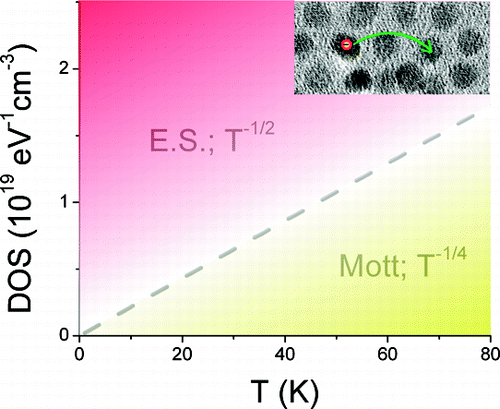
\includegraphics[scale=.50]{MottvsES.png}
\caption{Density of states vs Temperature. This plot describes the interface between ES and Mott transmission of electrons. (Graph courtesy of Heng Liu)}
\label{MvsES}
\end{center}
\end{figure}

\subsection{Coulomb Glass vs Artificial Nanosolids}
Coulomb glasses are the original substrate on which the ES model of electron conduction was based. The "glass" in coulomb glass refers to a phase in which electron-electron interactions impair conduction and dynamics become slow, like the flow of a glass~\cite{ortuno04}. Artificial nanosolids are arrays of granules which have a higher intra-granule conduction than a inter-granule conduction. The differences begin at the density of states. In artificial nanosolids, the density of states can be more creative. By changing the size of the granule, and the material it is made out of (metal, insulator, superconductor) the amount of available electron slots per site (and the energy of each slot) can be chosen. There are two energy scales for each grain. $\delta$ is the mean level spacing. $E_c$, the energy required to pack on one more electron onto a site is on the order of 3000 Kelvin ~\cite{glatz08} .The distances are also different. For coulomb glasses, the distances are basically the inter-atomic distances. There we are basically talking about electron jumps between atoms on a crystal lattice. As the name suggests, in artificial nanosolids the distances are arbitrary. For typical artificial nanosolid applications, we are in the nanometer to tens of nanometers range~\cite{beloborodov05}. While the general electric potential plays a role in both systems, It plays a bigger role in the coulomb glass since the scales are smaller and the electric potential scales as $1/r$.

\subsection{Inelastic vs. Elastic tunneling}
As well as blocking each other, electrons also can impart energy onto each other which may result in an electron being dislodged. This is referred to as inelastic co-tunneling. If instead the electron tunnels or otherwise travels without dislodging, it is referred to as elastic co-tunneling (see fig. ~\ref{inelasticvselastic}). For low to medium temperatures, the main tunneling mechanism will be elastic. At higher temperatures, we expect a transition to in-elastic tunneling~\cite{Glazman05}.

\begin{figure}[htbp]
\begin{center}
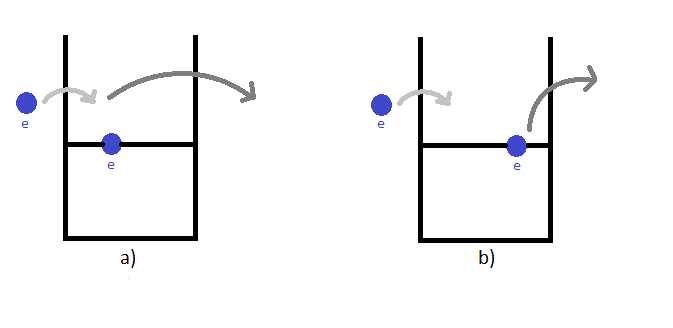
\includegraphics[scale=.50]{inelasticvselastic.png}
\caption{a) elastic transmission of electrons. b) inelastic transmission of electrons.}
\label{inelasticvselastic}
\end{center}
\end{figure}

\subsection{Temperature}

Temperature-dependent phase transitions are scattered throughout the spectrum and so it is important to specify at which temperatures we are working with. At temperatures lower than the Neel temperature, We encounter the first transition called "Mott-Heisenberg". At these low temperatures, the magnetic fields of the electrons have a chance to couple into anti-ferromagnetic pairs. Also, During tunneling events, electrons will avoid atoms which are occupied with other electrons of similar spins as sharing an atom would require an increase in energy compared to one of opposite spin ~\cite{Gebhard03}. At medium temperatures, we have a transition between elastic and inelastic. In order for an electron to land on an occupied site it must have enough energy to overcome the Coulomb blockade. This is only possible if it was given enough kinetic energy from a phonon (sufficient thermal energy). As the temperature is increased, electrons can begin stacking. Once an electron stacks onto another electron, Coulomb repulsion guarantees that either electron will quickly move on~\cite{Glazman05}. At much higher temperatures, the system starts to have enough free thermal energy to exceed the coulomb blockade energy. That is, the energy required to stack 2 electrons in the same quantum dot. This yields a crossover temperature which was discussed during our comparison of ES vs Mott systems ~\cite{aharony92}. Depending on the density of states, there will eventually be higher energy states on which to pack on electrons. For our purposes, we will stay in between these two systems. Our temperatures will be high enough that magnetic moments can be ignored, yet low enough that the maximum number of electrons allowed on the same quantum dot will be two.

\subsection{Density of States}
There are many methods of characterizing the energy of an electron. One of these is the density of states. This is a histogram of the energies that electrons can be in. For example in ~\ref{moundDoS}, there are many electrons at a relatively low energy and the number of electrons with higher energies decreases with energy. In ~\ref{crystalDoS} there is only one energy option for electrons. We see two peaks because the holes act as particles in that the system requires energy to move those as well. The value on the x axis is the energy required to fill or empty each hole or particle respectively. By knowing the shape of the density of states, one can discern important intricacies of a system. These can include the energy scales, the relaxedness, and the bandgap of a system. The typical kinetic energy of an electron in a fermi glass is $E = E_o + \frac{(\hbar k)^2} {2m}$. If one follows through the math, the dispersion relation ends up as $D_n(E) = \frac {nc_n} {p c^{n/p}_k} (E- E_o)^{n/p-1}$ ~\cite{Kittel96}. If the particle distribution is symmetric (same amount of electrons as holes) then the density of states will be symmetric, as long as the system is relaxed.

\begin{figure}[htbp]
\begin{center}
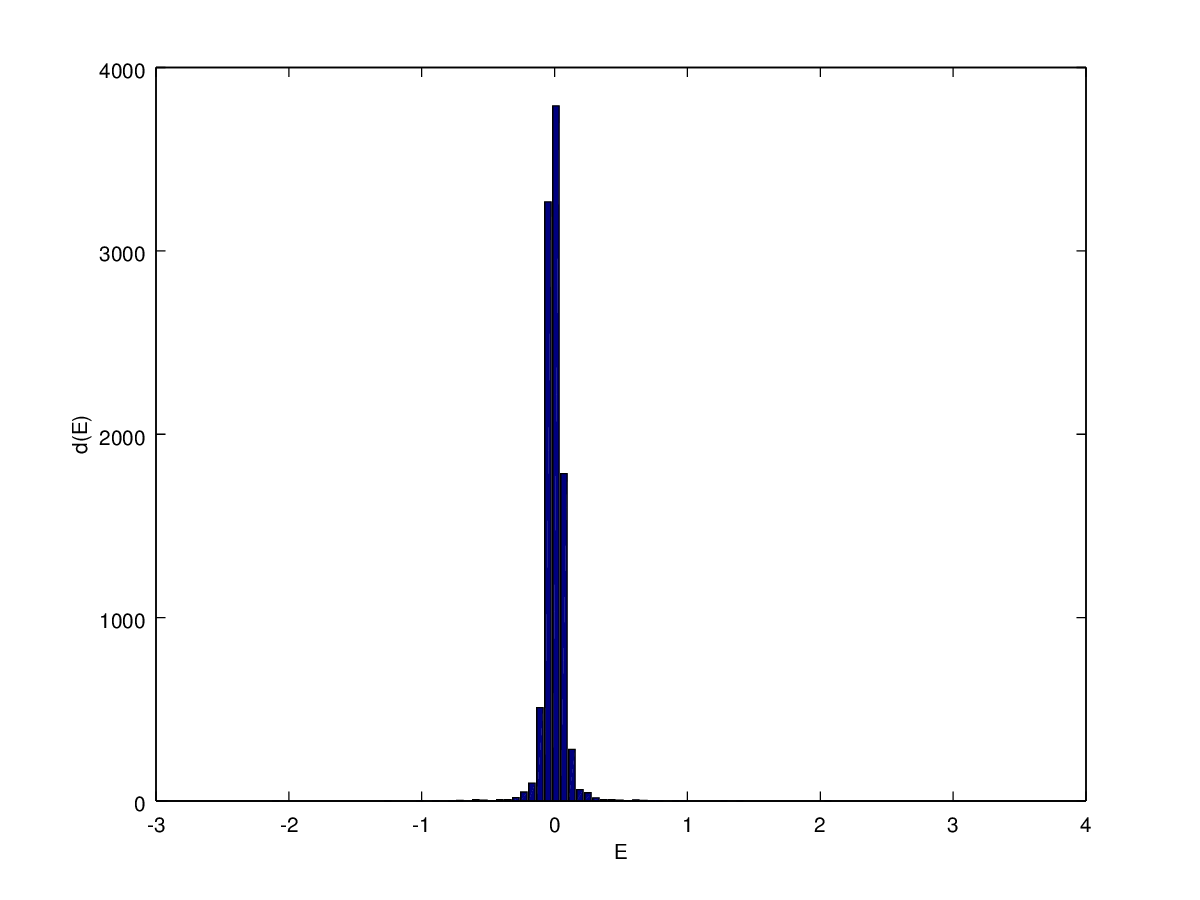
\includegraphics[scale=.50]{veryCloseDos.png}
\caption{The density of states for a system with a high amount of randomness in the energy.}
\label{moundDoS}
\end{center}
\end{figure}

\begin{figure}[htbp]
\begin{center}
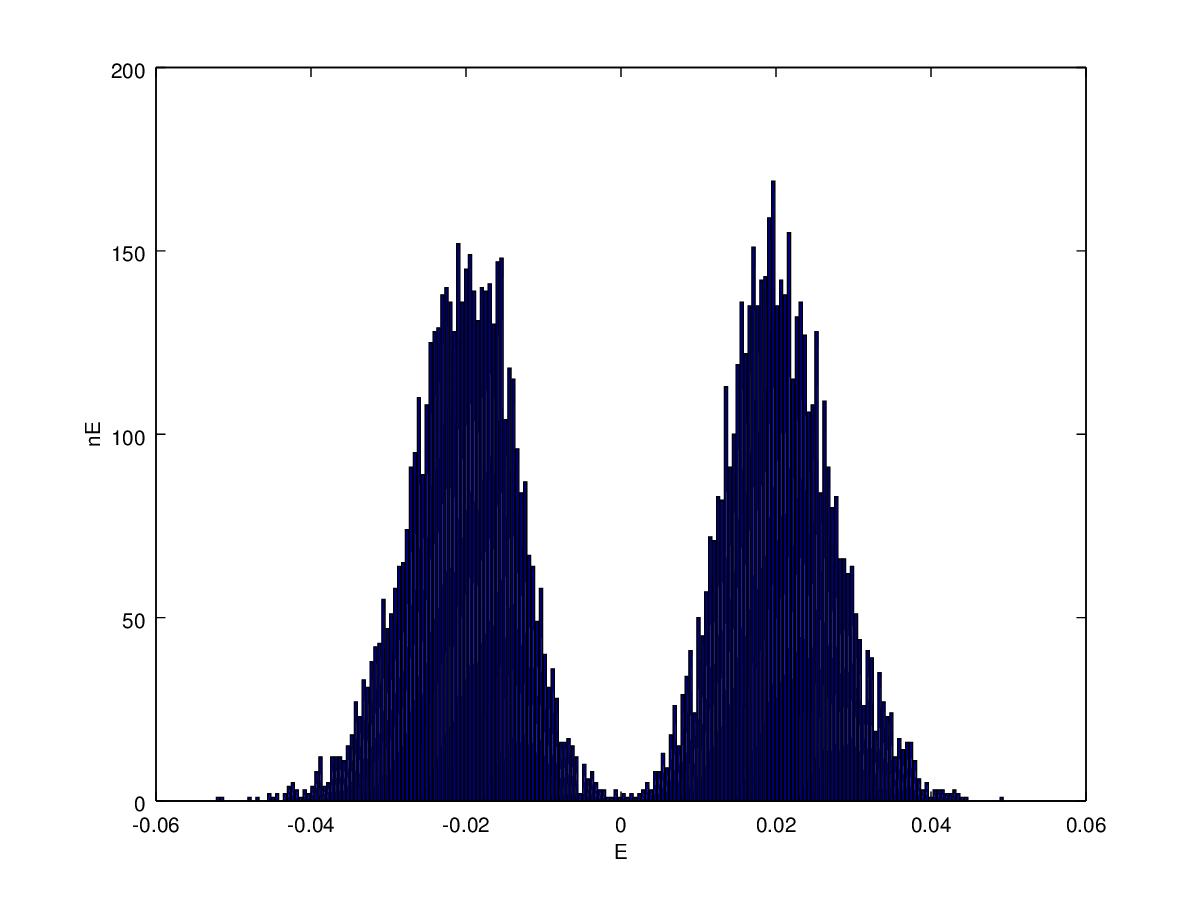
\includegraphics[scale=.50]{critDoS.png}
\caption{The density of states for a system where there is a critical amount of randomization and the two peaks are just beginning to touch.}
\label{critDoS}
\end{center}
\end{figure}


\begin{figure}[htbp]
\begin{center}
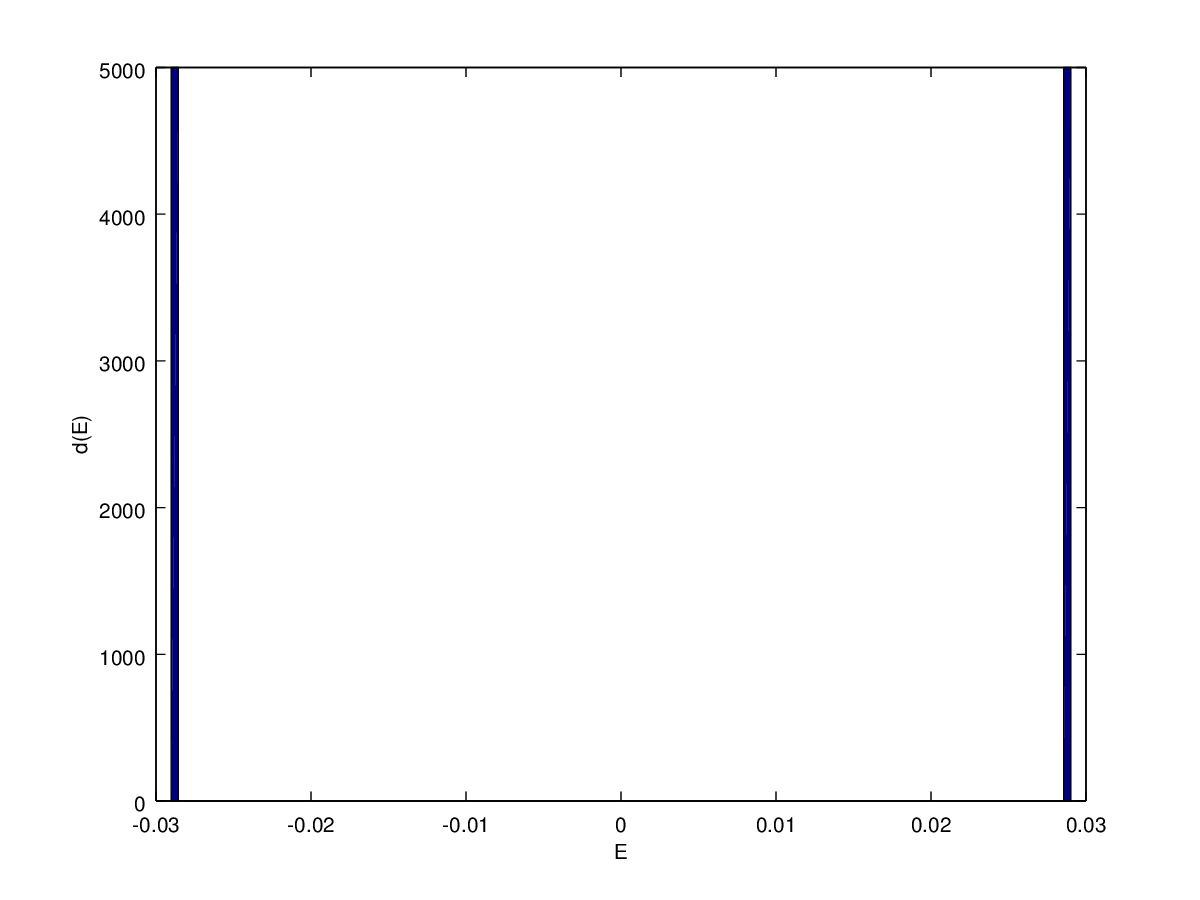
\includegraphics[scale=.50]{splitDos.png}
\caption{A low entropy system (Wigner crystal).}
\label{crystalDoS}
\end{center}
\end{figure}





%this file is deprecated and should be deleted

\chapter{Dias}		% chapter 1
\label{codechap}
\section{Dias}

\subsection{Monte Carlo Simulator}
{\sc dias} (Dynamics In Artificial Solids) is a code which at its heart is a Monte-Carlo simulator. {\sc dias} begins by taking in parameters such as granule-to-granule distance, number of electrons, number of lattice sites, number of time-steps, temperature, voltage bias, thermal gradient, material coefficient, and substrate potential variance. The granule-to-granule distance is on the order of 10 nanometeres. We have a square grid which is periodic. Variances in granule distances are uniformly introduced with limits according to user-set parameters. The number of electrons can vary between double-empty systems and double occupied sites. The number of time-steps is usually set to the square of the number of particles. This is to ensure a statistically justified result from the monte carlo aspect of the simulation. Temperature is set in Kelvin and is usually varied in the range where our material coefficient would give interesting results.  A positive voltage bias will act on a particle so that it is coerced to move upstream. Conversely, a positive voltage bias will force a hole to move downstream. This hints at a particular symmetry in which we chose for the simulation. Some previous studies have chosen to only focus on electron jumps and reject any jump that begins with a hole ~\cite{Ferrero14}. We decided to allow jump probabilities to be calculated from an electron hole's point of view as well. For current/voltage measurements, the system is periodic so that the current will just keep traveling at a steady pace. The code was also forked to a closed system to study thermoelectric properties. The memory choices we made are also worth mentioning. There were several arrays of data and keeping these to a minimum was important as memory management was an issue due to the limited space on GPU cards. We had between 1.5 and 2 Gb of memory to work with. These matrices include particle/hole, substrate potential, distance between sites, thermal gradient, and size of each granule. In order to maintain neutrality, the voltage bias was artificially set. This meant that the effective charge of a filled site was half an electron. If an electron were to move, the charge then became negative half and electron. The Monte-Carlo algorithm shows up twice to find the jump site.  First, a lattice site is chosen with probability according to it's energy. Second, the jump probabilities to each site are calculated using Eq.~\ref{probability} for said site. These probabilities are summed up and a number is chosen between 0 and that sum. This in turn gives a Monte-Carlo jump which is weighted by the jump probabilities. This jump is done and the system moves on to the next timestep under the new electron configuration. Meanwhile the properties of interest are measured. This repeats for the number of requested time steps. The pseudocode describing this process was outlined below:

\begin{varwidth}{\dimexpr\linewidth-2\fboxsep-2\fboxrule\relax}
\begin{algorithmic}[1]
\State Total = 0
\For {i = 1 to number of sites}
\State Total =+ $W_i$
\EndFor
\State newSum = 0
\State pick a random number R from 0 to Total
\For {i = 1 to number of sites}
\State newSum =+ $W_i$
\If {newSum $>$ R}
\State stop For loop, that is the jump site
\EndIf
\EndFor

This pseudocode is what is referred to as the "Tower Method". It is used in picking the starting particle as well as picking the particle to jump to. 
\end{algorithmic}
\end{varwidth}%

Originally we picked the starting particle randomly. Unfortunately in order to have a rejection-less system, this cannot happen. If it did, then particles which would have practically no chance of jumping would be moved with probability $ 1/N^2$. In order to fix this, we followed the algorithm posed in ~\cite{Newman99}. They propose first picking two particles with probabilities via the tower method,based on their energies. This way, particles which are less stable are moved more often. Because of the distance parameter in our probability, we are forced to pick one particle at a time. This way the second particle is picked based on the change of energy of the system, with a distance component. This algorithm allows for maximum parallelization and no rejection. The parallelized tower method is efficient as we can use a parallel prefix scan to stack the probabilities while also finding the maximum value in order to normalize. Doing a search for the right interval can also occur in parallel as each thread can be given a range, and the appropriate range can be found in log(N) time. 

\begin{varwidth}{\dimexpr\linewidth-2\fboxsep-2\fboxrule\relax}
\begin{algorithmic}[1]
\State number of slices = sizeArray/sharedMemory + 1
\State size of slice = sharedMemory
\State sumStart = 1
\For {i = 1 to number of slices}
\For {k = 1 to log(size of slice)}
\For { j = sumStart to size of slice/2}
\State add first half of slice to second half, put that sum in the second half
\EndFor
\State sumStart = size of slice/2
\State size of slice  = size of slice / 2
\EndFor
\EndFor
\State (now we stitch each shared memory together)
\State totalSum = 0
\For {i = 1 to number of slices}
\State totalSum = totalSum + sliceSum
\EndFor

This pseudocode is what is referred to as the "Parallel Reduction". It is device specific to GPGPU's, but can be generalized depending on "shared memory". This can be easily combined with a simple parallel sum to create a parallel dot-product algorithm. 
\end{algorithmic}
\end{varwidth}%


\subsection{Thoon Cluster}
This research was performed on a variety of machines, mostly consisting of Nvidia graphics cards. I had access to one stand-alone pc with a GTX 570, 8 pcs in a computer lab with GTX 570s, and 60 nodes with 2 GPU's each on the Gaea cluster in the computer science building. The Gaea cluster was powerful, but frequently busy such that only a third to an eighth was typically available. Meanwhile there was a computer lab with 8 linux based pcs, each with an Nvidia gtx 570. Unfortunately, they were barely on the same network. To remedy this, I wrote a script which divided up the parameter scans in the form of bash scripts and sent these to the respective computers. These then started the simulations and a timer in the form of a cron argument. The cron would then check every five minutes to see if the simulation was done. If so, then the data was sent back to the host computer. This had a few weaknesses, namely the clunkyness and the fact that one had to wait for the cron to trigger. This meant that short scans were impractical. Eventually this was all replaced with the free-lisence version of the Torque job scheduler. With the computers united into a small "cluster", running batches became more streamlined. This ad-hoc cluster is called THOON (Torque Hub On One Node). 

\subsection{GPU Algorithms}
The problem of electron hopping via Monte-Carlo algorithm can be solved very efficiently using parallel/GPU algorithms. In particular we use an algorithm called the "tower method" ~\cite{Krauth06}. Typically when one is doing a Monte Carlo study, there is an acceptance region and a rejection region ammong a range of choices. A choice is examined and it is either rejected or accepted. Using the tower method, all choices are stacked on top of each other (like a tower) and there is no rejection region. The first step, finding the probability to jump to each site is solved via the classical parallel scheme, where each lattice site can be individually calculated in its own thread. Once we have the probability matrix, we need to sum it in order to normalize it. This can be done via a parallel reduction algorithm. Taking advantage of on-board GPU memory, we can perform the reduction in O(N/P + log N ) time rather than O(N) time, where P is the number of GPU cores. Now that the system is normalized, we can roll a dice between 0 and 1 to find where the particle will go. We must then sum our probabilities until we find that number. This can be done with a parallel prefix sum. Parallel reduction and prefix sum algorithms were written and then replaced by Nvidia's more efficient Thrust functions. Thrust is a template library for CUDA which allows the implementation of high performance parallel applications.

\begin{varwidth}{\dimexpr\linewidth-2\fboxsep-2\fboxrule\relax}
\begin{algorithmic}[1]
\State First a nearest neighbor exchange
\For {i = 1 to number of sites}
\If {there's a particle at that site}
\State calculate energy without moving the particle:
\State {\textit{potential energy calculated everywhere}}
\State {\textit{sum reduction of the potential energy to one number (lets call it $S_1$) }}
\State test moving the particle up
\State {\textit{potential energy calculated everywhere}}
\State {\textit{sum reduction of the potential energy to one number (lets call it $S_2$) }}
\If {$S_1$ $>$ $S_2$}
\State leave the system
\Else
\State change it back
\EndIf
\State repeat for the other 3 directions (down,left,right)
\EndIf
\EndFor
\State The system is now slightly more relaxed
\State Now for switching highs and lows
\While {system is not relaxed}
\For {j = 1 to number of sites}
\State find the energy at each site normally:
\State {\textit{calculate potential,substrate, \& coulomb blockade energy everywhere. Sum and call this $S_3$}}
\State find the energy at each site with the particle removed (or added if the site was empty ):
\State {\textit{calculate potential,substrate, \& coulomb blockade energy everywhere. Sum and call this $S_4$}}
\State DosMatrix[j] = $S_4$ - $S_3$
\EndFor
\State {\textit{find lowest and highest values on the DosMatrix}}
\If {DosMatrix[index of lowest] + DosMatrix[index of highest] $<$ 0 }
\State swap particles
\Else
\State system is relaxed
\EndIf
\EndWhile
\end{algorithmic}
\end{varwidth}%

\subsection{Optimizations}
Various optimizations were done in order to speed up this code. Originally this was a linear CPU code, but obvious parallelisms made this code perfect for being run on a GPU. Still, there were some less obvious optimizations. One such optimization was previously discussed, moving to a rejection free system. In a rejection system, the particle has a high chance of staying at the same cell each turn. This means that a lot of computation is spent not gaining any valuable information. To fix this, we moved to the rejection free system (BLK?)~\cite{Newman99}. It is as if one jumped the simulation forward skipping all non-events. For one to do this, the system time must be kept. This is done by integrating all of the probabilities:
\begin{eqnarray}
\delta t = \frac {1} {\Sigma P_{\mu \rightarrow \nu}},
\label{systemTime}
\end{eqnarray}
where $\delta t$ is the change in system time, and $P_{\mu \rightarrow \nu}$ is the Markov transition matrix. Because of {\sc cuda} and algorithms like parallel reductions, it ends up being much faster to calculate this than to try to calculate all of the rejections. There were optimizations that skipped unnecessary calculations. One of these was the calculation of the potentials after a particle is moved. The naive way to do this would be to recalulate all of the potentials from each particle. The optimized way to do this would be to use a crater-mound system. That is, only focus on the effects due to the particle that has moved. In other words, add a crater to the potential around the site where a particle left and add a mound in the potential around the site where the particle has appeared. Another optimization was the 4D lattice matrix. 

\subsection{The Lattice}
While the easiest system to model would have been a square lattice, This would have left out a large amount of interesting phenomena. To incorporate this, we started out with a square lattice and then gave each site a certain $\delta x$ or $\delta y$ variance. There are a few ways to then use this kind of implementation. The first one would have been to then calculate the distances from one site to another on the fly, possibly approximating for further away site. The way that we picked to do this was to hold all of the distances from one site to another in a 4D matrix (a matrix of distances for every site on the grid). This has the advantage that no calculations have to be run at each GPU core. Since the calculation of distance involves a square root, this would have been heavy on the workload. The disadvantage is that for a $100 \times 100 $ system, we require $100 \times 100 \times 4$ bytes of data (or 400MB using the float type). Fortunately, NVIDIA GTX 570 cards have at least 1200 megabytes of memory, so this did not end up being an issue.

\subsection{Distance-substrate correlation}
In the physical world, this system is not a grid, but rather a dense packing of granules. This can be imagined as a 2D packing of variously sized orbs. One can then see that the distance between orb centers will depend on the size of the neighboring orbs. For ease of algorithms, we took this correlation in the opposite direction. The size of an orb is defined by half the distance to the nearest orb. The substrate potential is also affected by this. Granule size randomness did not have much effect on the system directly. This is because it only affects how much energy it takes to pack two electrons on the same granule. If the granule is bigger, the electrons do not have to sit so close together and the charging energy is lowered. But the issue is that even with a larger granule, the temperature required to pack two electrons onto the same granule is still in the thousands of Kelvin and outside of the scope of this study. The correlation's effect on substrate randomness however did come into effect, as small changes in the substrate potential can have large effects on the density of states.

\subsection {Density of States}
The energy involved when removing or adding a particle to a lattice site is what determines the probability to jump to it. It then makes sense to ask what the distribution of potential energies will be. The purpose of this code was not originally to determine the density of energy states of an electron lattice. Nevertheless it serves two practical purposes. First, it helps to make sure that the particular energy contributions are balanced accordingly. Looking at the density of states, one can immediately associate characteristics to electrical potential, substrate potential, etc. Then, at a glance, one can quickly determine if the substrate potential is too strong and is washing out electric potential contributions. The second purpose is to assure that a particular system is fully relaxed before simulations begin. Due to the inherent randomness of the system, particular outcomes may sharply vary depending on the initial conditions. Assuring that the system is relaxed before starting can compensate for this. One clue that the system is relaxed is that in two dimensions, there will be a linear (absolute value) pattern near 0 in the density of states. We use a previously determined algorithm in order to quickly relax our system ~\cite{Vinokur08}. We begin with a nearest-neighbor comparison of every particle site and moving them if the overall energy is lower. Then we find the particle which is imparting the most potential energy by existing. This is compared to the hole for which filling it would cause the most potential energy to be added to the system. If the two energies, when summed, are less than the original, then the switch is performed. The area around each switched particle is then scanned to see if any readjustments can be made to further lower the potential energy of the system. The density of states is then measured again everywhere and the process is repeated until the energy can no longer be reduced. The valley in the density of states can also be characterized. If the slope near $E=0$ is linear, then we know we are looking at a 2D system. If it is parabolic, then this signifies a 3D system. As a benchmark, we analyzed our valley slope and found it to agree with the 2D system characterization. 

\subsection{Algorithmic Benchmarking}
The average jump distance for a high temperature system should be ~0.69614 spaces. This matches to within $1\%$ accuracy with my results of 0.68943 spaces. This difference is negligible considering the statistical variation of any Monte Carlo system. The expected jump distance was found via Monte Carlo integrator. First, the values of Eq.~\ref{probability} were found at a grid of points with similar spacing to what we use in the simulation. Second, particles were dropped onto this grid depending on the function values a-la Monte Carlo method. Third, the mean jump distance was calculated via the first moment equation
\begin{eqnarray}
\bar r = \frac {\sum r \cdot n} {\sum n}, 
\label{firstMoment}
\end{eqnarray}
where $r$ is the distance from the center of the grid cell, and $n$ is the number of particles at each grid cell. The parameters for this comparison were fairly basic. The temperature was 1 degree kelvin, there was no external current, the system size was 100x100, and there was only one particle. Multiple particle comparisons have been done, but because the jump probabilities are different depending on wether the site is empty or full, the comparison becomes much more complicated. The point of this benchmark was to make sure the complicated GPU Monte-Carlo integrator was working as expected. With 3 major components to this system, (calculating the energies, calculating the weights from the energies, and calculating a jump site from the weights), this was a simple way to make sure everything was working together properly. Creating simple scripts to test more complicated scripts also became a useful tool in other parts of the research. For example, studying the behavior of the energy as a function of distance can be done via the Dias simulator, and outputs can be output for testing. But this can be complicated and the program may need to be changed and re-compiled in between tests. By writing a simple function grapher in Octave and tuning the same parameters, the interaction between different energy sources could be observed more closely.

\subsection{Results}
  Other results also followed the expected trends. In Fig.~\ref{TvsRbar} , One can see that as the temperature rises, the system slowly kills any aditional help from the $E_{ij}$ component and it asymptotes to the jump distance related to the locality of the electron. In Fig.~\ref{JvsV} , The dependance of current on voltage is almost exponential. In Fig.~\ref{TvJ}, one can see how the electrons can't go as far once the temperature is increased. A modified version of the simulator was run to explore the physics of electron transport as the system becomes saturated. The number of electrons in the system was slowly increased and simulations were run at different numbers of particles. In ~\cite{Beloborodov07} they give approximate jump distances at various temperatures. We duplicated these and found similar values for $\bar \mu = .01$ and $\delta xy = .45$.

\begin{figure}[htbp]
\begin{center}
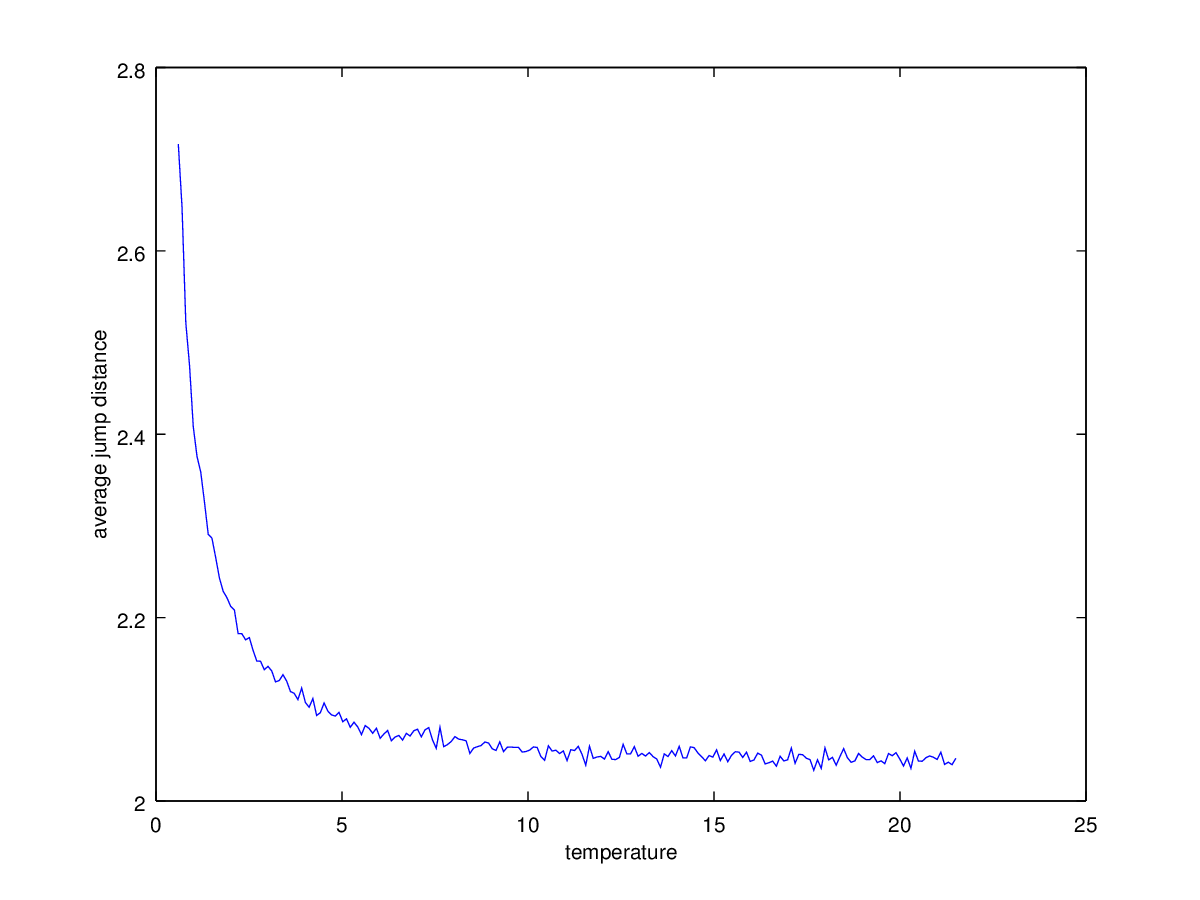
\includegraphics[scale=.50]{TvsRbar.png}
\caption{Temperature vs average jump distance .}
\label{TvsRbar}
\end{center}
\end{figure}

\begin{figure}[htbp]
\begin{center}
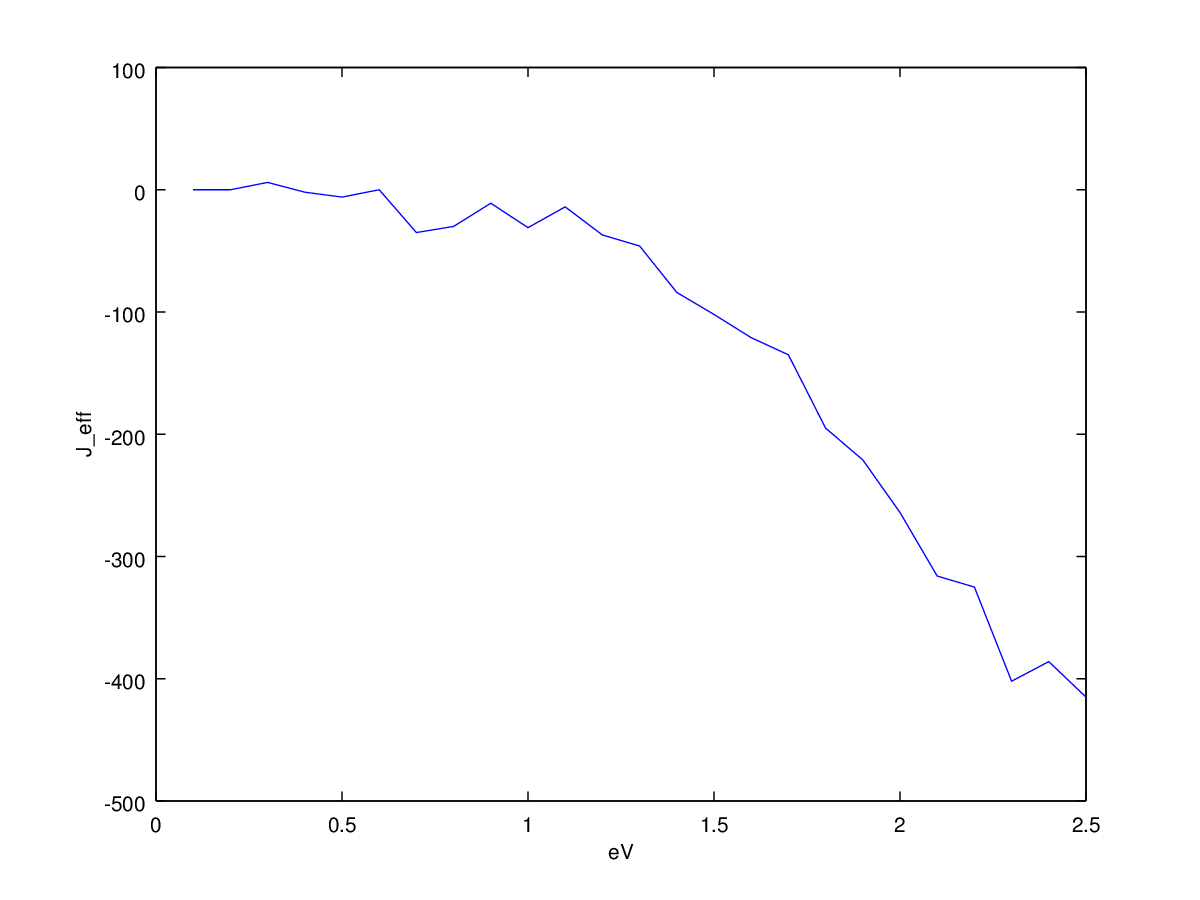
\includegraphics[scale=.50]{JvsV.png}
\caption{Current vs Voltage .}
\label{JvsV}
\end{center}
\end{figure}

\begin{figure}[htbp]
\begin{center}
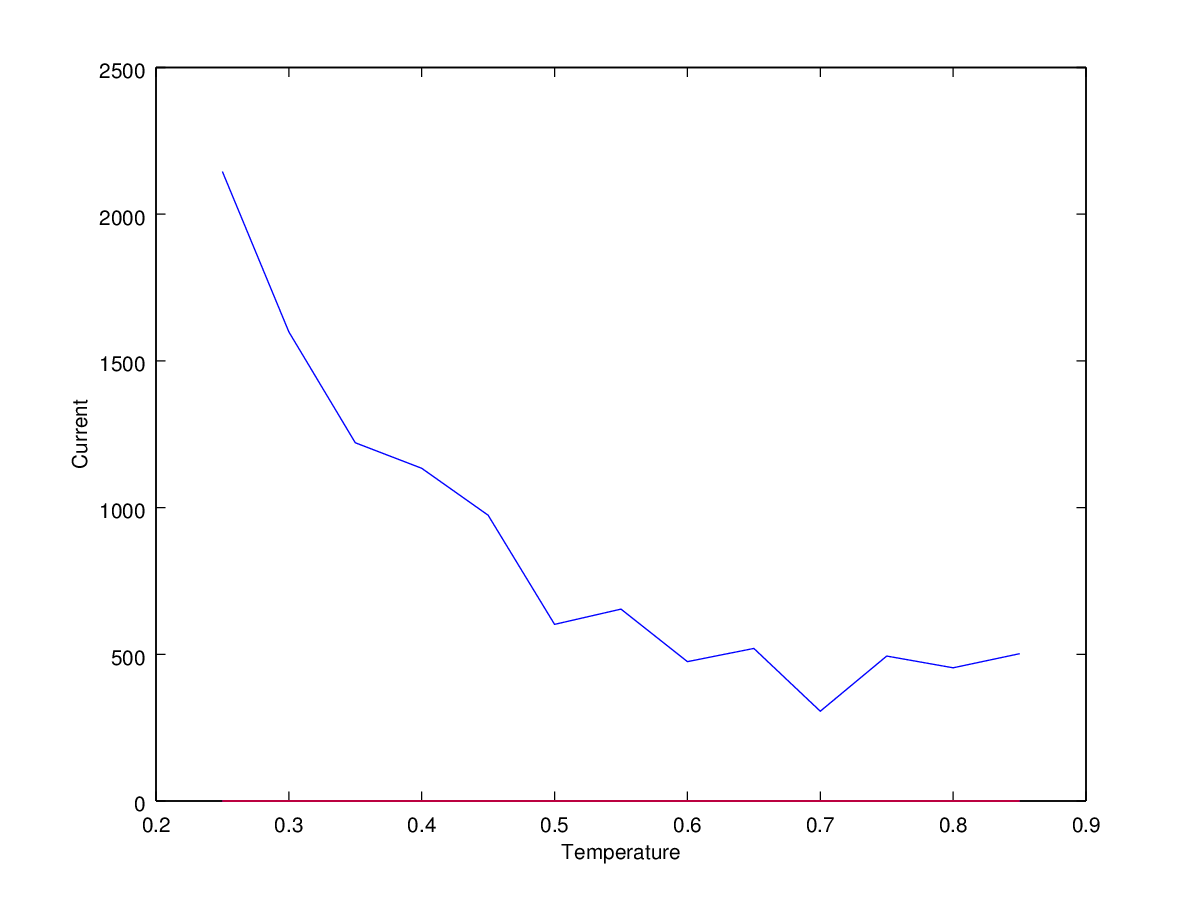
\includegraphics[scale=.50]{JvT.png}
\caption{Temperature vs current .}
\label{TvJ}
\end{center}
\end{figure}


%this file is deprecated and should be deleted

\begin{thebibliography}{10}
\bibitem{mott72} Mott, N. F.; Peierls, R. (1937). "Discussion of the paper by de Boer and Verwey". Proceedings of the Physical Society 49 (4S): 72

\bibitem{efros75} A L Efros and B I Shklovskii , J. Phys. C8, L49 (1975)

\bibitem{glazman05} L.I. Glazman, M. Pustilnik, in "Nanophysics: Coherence and Transport," eds. H. Bouchiat et al. (Elsevier, 2005), pp. 427-478

\bibitem{kirkengen09} M. Kirkengen , J. Bergli, "Slow relaxation and equilibrium dynamics in a two-dimensional Coulomb glass: Demonstration of stretched exponential energy correlations" PHYSICAL REVIEW B 79, 075205 2009

\bibitem{aharony92} A. Aharony, Y. Zhang, M.P. Sarachik, "Universal Crossover in Variable Range Hopping with Coulomb Interactions", Physical Review Letters 1992

\bibitem{joung} D. Joungand, S. Khondaker, "Efros-Shklovskii variable range hopping in reduced graphene oxide sheets of varying carbon sp2 fraction", http://arxiv.org/pdf/1210.1876.pdf

\bibitem{glatz09} A. Glatz, I. Beloborodov, "Thermoelectric and Seebeck coefficients of granular metals", PHYSICAL REVIEW B 79, 235403 2009

\bibitem{chen} L. Chen, S. Gao, X. Zeng, A. Mehdizadeh Dehkordi,T. M. Tritt,and S. J. Poon, "Uncovering High Thermoelectric Figure of Merit in (Hf,Zr)NiSn Half-Heusler Alloys" , http://arxiv.org/pdf/1505.07773.pdf

\bibitem{ortuno04} M. Ortuno , A. Somoza, "Coulomb Glasses", http://www.lancaster.ac.uk/users/esqn/windsor04/docs/artuno-cg.pdf

\bibitem{beloborodov05} I. S. Beloborodov, A. V. Lopatin, F. W. J. Hekking, R. Fazio, and V. M. Vinokur , "Thermal transport in granular metals ",Europhys. Lett. 69, 435 (2005)

\bibitem{glatz08} A. Glatz ,I. S. Beloborodov , "Nanogranular Thermoelectrics" , http://arxiv.org/pdf/0810.5545.pdf

\bibitem{Gebhard03} B. Gebhard, "The Mott Metal-Insulator Transition: Models and Methods", Springer 2003

\bibitem{Glazman05} L. Glazman, M. Pustilnik, "Low-Temperature Transport Through A Quantum Dot", http://arxiv.org/pdf/cond-mat/0501007v2.pdf

\bibitem{Liu10} H. Liu, A. Pourret, P. Guyot-Sionnest, "Mott and Efros-Shklovskii Variable Range Hopping in CdSe Quantum Dots Films", ACS Nano, 2010, 4 (9), pp 5211-5216

\bibitem{Vinokur08} A. Glatz, V. Vinokur, J. Bergli, M. Kirkengen, Y. Galperin, "The Coulomb gap and low energy statistics for Coulomb glasses", Journal of Statistical Mechanics: Theory and Experiment, 2008

\bibitem{Kittel96} C. Kittel, "Introduction to Solid State Physics", Wiley, 1996

\bibitem{Beloborodov07} I. Beloborodov, A. Lopatin, V. Vinokur, K. Efetov, "Granular Electronic Systems", Reviews of Modern Physics, Volume 79, April-June 2007

\bibitem{Sadovskyy14} I. Sadovskyy, A. Koshelev, C. Phillips, D. Karpeev, A. Glatz, "Stable large-scale solver for Ginzburg-Landau equations for superconductors", Journal of Computational Physics, 09/2014

\bibitem{Ferrero14} E. Ferrero, A. Kolton, M. Palassini, "Parallel kinetic Monte Carlo simulation of Coulomb glasses" ,arXiv:1407.5026

\bibitem{Krauth06} W. Krauth, "Statistical Mechanics: Algorithms and Computations", Oxford University Press, Oxford, 2006, pp. 33–34

\bibitem{Newman99} M. Newman, G. Barkema, "Monte Carlo Methods in Statistical Physics", Oxford University Press, Oxford, 1999, pp. 41-42

\bibitem{Sparks16} T. Sparks, M. Gaultois, A. Oliynyk, J. Brgoch, B. Meredig, "Data mining our way to the next generation of thermoelectrics", Scripta Materialia, Volume 111, 15 January 2016, Pages 10–15

\bibitem{Chandra??} R. Chandra, "Mechanical vapour compression refrigeration", Refrigeration and Air Conditioning, New Delhi, India: PHI Learning. p. 3. ISBN 81-203-3915-0.

\bibitem{Brown63} J. Brown, "Thermodynamics of a Rubber Band", American Journal of Physics, 31 (5): 397–397, May 1963, doi:10.1119/1.1969535

\bibitem{Miszczak15} M. Miszczak, "GINZBURG-LANDAU SIMULATIONS OF NARROW SUPERCONDUCTING STRIPS" , Northern Illinois University, Department of Physics, 2015

\end{thebibliography}

%%%%%%%%%%%%%%%%%%%%%%%%%%%%%%%%%%%%%%%%%%%%%%%%%%%%%%%%%%%%%%%%%%%
%%  Appendices

\appendix
\chapter{Objective Symptoms}
% \OnePageChapter	% (use if this chapter/appendix is 1 page long)

Appendices follow the same page-numbering rules as regular chapters. The first
page of a multi-page appendix is not numbered. But the page of a
single-page appendix {\em is} numbered.

\textbf{Are they slow learners} or is it a \emph{REAL} problem?
These are classic findings in the hopelessly computer challenged.

\begin{enumerate}

\item  Can't copy from hard drive to disk.
\item  Can't eject disks.
\item  The word ``disk'' has thousands of meanings to them. None are correct.
\item  Saving a document in any form is a concept totally unexplainable to them.
\item  Desktop covered with Untitled Folders - look again,
		untitled folders are everywhere.
\item  ``Lost'' documents found often in the Apple Menu.
\item  Trash always full. Claim they don't know how to place things in trash.
\item  Mysterious things happen to their documents or computer
	when they are not present.  AKA ``computer victims''.
\item  Highlighting = deleting. Dragging = Oblivion.
\item  Selecting, double-clicking a problem?
		They will always say their mouse is broken.
\item  Their double- click mechanics wants you to send them to a neurologist.
\item  Computer always on due to fear of having to restart it.
\item  Have never read their QuickMail - will say ``I prefer a phone call''.
\item  Have magical beliefs about what computers do.
\item  Describes some flaky way computers could REALLY help them,
		but is not yet available.
\item  Constantly saying they need more ``memory''.
\item  Requests gizmos and gadgets, i.e., ``mouse leash'' or ``disk cozy''.
\item  Avoids eye contact when talking about computers.

\end{enumerate}
			% file with Appendix A contents
\chapter{Ode to Spot}

\noindent\paragraph{(Data, Stardate 1403827)}
Throughout the ages, from Keats to Giorchamo, poets have
composed ``odes'' to individuals who have had a profound effect
upon their lives.  In keeping with that tradition
I have written my next poem \ldots in honor of my cat.
I call it\ldots{}Ode\ldots{}to Spot.
(Shot of Geordi and Worf in audience,
looking mystified at each other.)

\begin{quotation}
\noindent Felus cattus, is your taxonomic nomenclature \\
an endothermic quadruped, carnivorous by nature? \\
Your visual, olfactory, and auditory senses \\
contribute to your hunting skills, and natural defenses. \\
I find myself intrigued by your sub-vocal oscillations, \\
a singular development of cat communications \\
that obviates your basic hedonistic predilection \\
for a rhythmic stroking of your fur to demonstrate affection. \\
A tail is quite essential for your acrobatic talents; \\
you would not be so agile if you lacked its counterbalance. \\
And when not being utilized to aid in locomotion, \\
It often serves to illustrate the state of your emotion.
\end{quotation}


\noindent(Commander Riker begins to applaud, until a
glance from Counselor Troi brings him to a halt.)
Commander Riker, you have anticipated my denouement.
However, the sentiment is appreciated.  I will continue.


\begin{quotation}
\noindent O Spot, the complex levels of behavior you display \\
connote a fairly well-developed cognitive array. \\
And though you are not sentient, Spot, and do not comprehend \\
I nonetheless consider you a true and valued friend.
\end{quotation}
			% file with Appendix B contents

\end{document}
